% Tekijä:   Teemu Likonen <tlikonen@iki.fi>
% Lisenssi: Creative Commons Nimeä-JaaSamoin 4.0 Kansainvälinen (CC BY-SA 4.0)
%           https://creativecommons.org/licenses/by-sa/4.0/legalcode.fi

\chapter{Rakenne ja sisältö}

Tämä luku on oppaan kaikista luvuista kenties käytännönläheisin. Luku
keskittyy asioihin, joita kirjoittaja miettii erityisesti dokumentin
sisällön kirjoitusvaiheessa. Kirjoittaja tekee esimerkiksi valintoja
otsikoinnin ja muun jäsentämisen osalta. Hän miettii tiedon esittämistä
paitsi tekstin avulla myös esimerkiksi luetelmien, kuvien ja taulukoiden
avulla. Kirjoittaja tekee myös typografisia valintoja tekstin muotoilun
ja korostuskeinojen näkökulmasta. Edellä mainittuja ja muitakin
dokumentin rakenteen ja sisällön asioita käsitellään niin tekniikan kuin
typografiankin näkökulmasta.

\section{Tekstikappaleet}
\label{luku:kappale}

Tekstikappale on tekstin osa, jonka pitäisi käsitellä suunnilleen yhtä
asiakokonaisuutta. Se voi olla esimerkiksi yksi aihe, näkökulma,
ajankohta tai henkilö. Tekstin seuraava kappale käsittelee jotakin
toista aihetta, näkökulmaa tms. Kappaleen vaihtuminen on lukijalle
merkki siitä, että tekstin sisällössäkin jokin muuttuu.

Latexin lähdetiedostoissa kappaleen vaihtuminen ilmaistaan
kirjoittamalla kappaleiden väliin vähintään yksi tyhjä rivi. Tätä
merkintäkielen piirrettä käsitellään myös luvussa
\ref{luku:kappaleen_vaihtuminen}. Kappale vaihtuu myös komennolla
\komentom{par}, joka sopii käytettäväksi esimerkiksi komentojen
määrittelyssä (luku \ref{luku:komennot}), kun halutaan varmistaa
kappaleen vaihtuminen tietyssä kohdassa.

Ladotuissa teksteissä kuten kirjoissa ja lehdissä kappaleen vaihtuminen
ilmaistaan melkein aina siten, että uuden kappaleen ensimmäinen rivi
sisennetään hieman. Niin on tässäkin oppaassa. Toisinaan tekstikappaleet
erotetaan pystysuuntaisella välillä, ja silloin kappaleiden ensimmäistä
riviä ei sisennetä. Kappaleiden välejä, sisennyksiä, rivien tasaamista
ja muita asetuksia käsitellään seuraavissa alaluvuissa.

Monissa kappaleisiin liittyvissä asetuksissa tarvitaan Texin mittoja ja
mittayksiköitä. Mittoihin liittyvää tekniikkaa käsitellään tarkemmin
luvussa \ref{luku:mitat}, joka on syytä tuntea ennen tämän alaluvun
lukemista.

\subsection{Tasaaminen ja palstan muoto}
\label{luku:kappaleen_tasaus}

Perusdokumenttiluokissa (luku \ref{luku:perusdokumenttiluokat})
tekstikappaleet tasataan oletuksena palstan molempiin reunoihin, ja tätä
palstan muotoa kutsutaan tasapalstaksi. Se tarkoittaa samalla sitä, että
rivillä olevia sanavälejä venytetään sopivasti, jotta jokainen rivi
näyttäisi yhtä pitkältä ja palstan molemmat reunat tasaiselta.

Käytännössä sanavälien venymiselle on määritelty yläraja, jonka yli
niitä ei venytetä. Ylärajan tarkoituksena on estää liian suuret ja rumat
sanavälit. Rajoitus on sinänsä järkevä, mutta se voi myös johtaa siihen,
että Tex ei saa tasattua kaikkia tekstikappaleita palstan oikeasta
reunasta: jotkin rivit yltävät palstan reunan yli; jotkin rivit jäävät
vajaaksi. Näin käy usein varsinkin suomen kielessä, jonka sanat ovat
usein pitkiä ja riveillä on vähänlaisesti sanavälejä. Suomen kielessä
sanavälien venymisen yläraja on usein tarpeellista asettaa oletusarvoa
suuremmaksi. Se tehdään mitan \mitta{emergencystretch} avulla,
esimerkiksi seuraavasti:

\komentoi{setlength}
\mittai{emergencystretch}
\begin{koodilohkosis}
  \setlength{\emergencystretch}{1em}
\end{koodilohkosis}

Kaikenlaiset kappaleiden latomiseen liittyvät tekniset rajoitukset voi
poistaa tai asettaa hyvin suuriksi komennolla \komentom{sloppy}. Komento
asettaa muun muassa sanavälien venymisen ylärajaksi 3\,em. Tämän
komennon käyttö ei ole kovin suositeltavaa, koska sillä on muitakin
seurauksia ja se voi vaikuttaa myös sellaisiin kappaleisiin, jotka
muuten saataisiin ladottua nätisti. Parempi on asettaa vain mitta
\mitta{emergencystretch} riittävän suureksi. Sanavälien venymiseen ja
kappaleiden tasaiseen latomiseen liittyvät asetukset voi palauttaa
oletusarvoihin komennolla \komentom{fussy}.

Hyvin tavallista on tasata teksti pelkästään vasempaan reunaan, jolloin
rivien pituudet vaihtelevat ja oikealla on niin sanottu liehureuna.
Oikea liehureuna sopii pitkiin teksteihin yhtä hyvin kuin tasapalstakin,
mutta se on parempi valinta erityisesti silloin, kun palsta on kapea.
Nimittäin kapealla palstalla venyviä sanavälejä on käytettävissä hyvin
vähän ja oikean reunan tasaaminen vaatii sanavälien venyttämistä joskus
kohtuuttoman paljon. Tekstiin jää rumia aukkoja.

\providecommand{\rivi}{}
\renewcommand{\rivi}[3]{\komento{#1} & \ymparisto{#2} & #3 \\}

\leijutlk{
  \begin{tabular}{lll}
    \toprule
    \ots{Komento} & \ots{Ympäristö} & \ots{Merkitys} \\
    \midrule
    \rivi{raggedright}{flushleft}{vasen tasaus, oikea liehu}
    \rivi{raggedleft}{flushright}{oikea tasaus, vasen liehu}
    \rivi{centering}{center}{keskitetty}
    \midrule
    \rivi{RaggedRight}{FlushLeft}
    {vasen tasaus, oikea liehu, tavutus (\paketti{ragged2e})}
    \rivi{RaggedLeft}{FlushRight}
    {oikea tasaus, vasen liehu, tavutus (\paketti{ragged2e})}
    \rivi{Centering}{Center}{keskitetty, tavutus (\paketti{ragged2e})}
    \rivi{justifying}{justify}{tasapalsta, tavutus (\paketti{ragged2e})}
    \bottomrule
  \end{tabular}
}{
  \caption{Tekstikappaleen tasaamiseen ja palstan muotoon vaikuttavat
    komennot ja ympäristöt. Osa sisältyy \paketti{ragged2e}\-/pakettiin}
  \label{tlk:kappaleen_tasauskomennot}
}

Kappaleiden tasaamiseen ja palstan muotoon vaikuttavia komentoja ja
ympäristöjä on koottu taulukkoon \ref{tlk:kappaleen_tasauskomennot}.
Taulukossa on mainittu ensin Latexin omat komennot ja sitten
\paketti{ragged2e}\-/paketin\avctan{ragged2e} vastaavat. Latexin omat
komennot estävät sanojen tavuttamisen, kun taas \paketti{ragged2e}\-/
paketin komennot sallivat tavutuksen normaalisti.

\subsection{Pystysuuntaiset välit}
\label{luku:pystysuuntaiset_valit}

Kappaleiden väliin ladottava pystysuuntainen tyhjä tila asetetaan mitan
\mittam{parskip} avulla. Se on oletuksena nolla, mutta pientä venymistä
kuitenkin sallitaan, eli joissakin tilanteissa kappaleiden väliin
voidaan latoa pieni tyhjä tila. Jos tyhjää tilaa ei haluta missään
tilanteessa, asetetaan mitta vain nollaksi:

\komentoi{setlength}
\mittai{parskip}
\begin{koodilohkosis}
  \setlength{\parskip}{0ex}
\end{koodilohkosis}

Seuraava esimerkkikomento asettaa kappaleväliksi 1,3\,ex. Lisäksi se
sallii kappalevälin venyä 0,2\,ex:n verran tai kutistua 0,1\,ex:n
verran.

\komentoi{setlength}
\mittai{parskip}
\begin{koodilohkosis}
  \setlength{\parskip}{1.3ex plus .2ex minus .1ex}
\end{koodilohkosis}

Silloin kun kappaleet ladotaan erilleen toisistaan, on yleensä hyvä
sallia kappalevälin venyä tai kutistua hieman, koska venyvät
pystysuuntaiset välit antavat Texille paremmat mahdollisuudet latoa
hyvännäköisiä sivuja. Venyvien välien avulla esimerkiksi sivun
tekstialueen ylä- ja alareunat saadaan aina samalle kohdalle. Toisaalta
myös liian suuret ja toisistaan liiaksi poikkeavat kappalevälit voivat
olla rumannäköisiä.

Tavallista kappaleväliä suurempien pystysuuntaisten välien tekemiseen on
olemassa kolme valmista komentoa: suuremmasta pienempään ne ovat
\komentom{bigskip}, \komentom{medskip} ja \komentom{smallskip}. Ne
sopivat käytettäväksi yksittäisiin tilainteisiin, joissa normaali
kappaleväli on liian vähän. Jos sivunvaihto osuu näiden komentojen
kohdalle, mitään väliä ei ladota sivun loppuun eikä seuraavan alkuun.

Edellä mainittujen komentojen latoman välin suuruuteen voi vaikuttaa
mittojen \mitta{bigskipamount}, \mitta{medskipamount} ja
\mitta{smallskipamount} avulla. Seuraavassa on esimerkkikomennot
mittojen määrittelemiseen ja samalla niiden oletusarvot:

\komentoi{setlength}
\mittai{bigskipamount}
\mittai{medskipamount}
\mittai{smallskipamount}
\begin{koodilohkosis}
  \setlength{\bigskipamount} {12pt plus 4pt minus 4pt}
  \setlength{\medskipamount}  {6pt plus 2pt minus 2pt}
  \setlength{\smallskipamount}{3pt plus 1pt minus 1pt}
\end{koodilohkosis}

Komentojen \komento{bigskip}, \komento{medskip} ja \komento{smallskip}
sijasta voi käyttää myös komentoja \komentom{bigbreak},
\komentom{medbreak} tai \komentom{smallbreak}. Nämä toimivat lähes
samalla tavalla, mutta niihin sisältyy myös sivunvaihtovihje. Toisin
sanoen ne vaikuttavat ladonta\-/algoritmiin siten, että komennon
kohdalla todennäköisyys sivun vaihtumiselle kasvaa suhteessa muihin
kohtiin. Sivu voi edelleen vaihtua muustakin kohdasta, jos algoritmi
löytää omasta mielestään vielä paremman paikan.

Pystysuuntaisten välien yleiskomento on \komentom{vspace}, jolle
annetaan argumentiksi välin suuruus ja mahdolliset venymisen rajat.
Tämäkin komento jättää välin latomatta, jos se sattuu sivunvaihdon
kohdalle. Sen sijaan tähdellinen versio \komentom{vspace*} latoo välin
joka tapauksessa, vaikka se olisi sivun lopussa tai alussa.

\komentoi{vspace}
\begin{koodilohkosis}
  Tekstikappale.
  \vspace{5ex plus 1ex minus .5ex}

  Toinen tekstikappale.
\end{koodilohkosis}

Komento \komentom{addvspace} toimii lähes samoin kuin \komento{vspace},
mutta se huomioi mahdolliset peräkkäiset \komento{addvspace}\-/ komennot
ja varmistaa, että vain suurin väli toteutuu. Jos siis useita
\komento{addvspace}\-/ komentoja sattuu peräkkäin, niiden määrittämiä
välejä ei ladota peräkkäin vaan ainoastaan suurin niistä ladotaan.
Seuraava esimerkki latoo kappaleiden väliin 2\,ex:n suuruisen
pystysuuntaisen välin:

\komentoi{addvspace}
\begin{koodilohkosis}
  Tekstikappale.

  \addvspace{1ex} \addvspace{2ex} \addvspace{.5ex}
  Toinen tekstikappale.
\end{koodilohkosis}

Jos edellisessä esimerkissä olisi käytetty \komento{vspace}\-/ komentoa,
pystysuuntaisen välin suuruus olisi 3,5\,ex, joka on välien
yhteenlaskettu suuruus.

\komento{addvspace}\-/komento soveltuu hyvin komentojen ja ympäristöjen
määrittelyyn (luvut \ref{luku:komennot} ja \ref{luku:ymparistot}).
Esimerkiksi itse määritellyn ympäristön alussa ja lopussa voi
\komento{addvspace}\-/ komennolla varmistaa tietynsuuruisen välin, mutta
jos sama tai muu vastaava ympäristö on dokumentissa kahdesti peräkkäin,
huomioidaan pystysuuntainen väli vain kerran eli suurimman välin mukaan.
Jotkin Latexin valmiit ympäristöt tekevät juuri näin eli käyttävät
\komento{addvspace}\-/komentoa välien asettamiseen.

Sivun alueella äärettömästi venyvän pystysuuntaisen välin saa komennolla
\komentom{vfill}. Mitan luonnollinen arvo on nolla, mutta se voi venyä
niin, että se täyttää kaiken tyhjän tilan sivulla. \komento{vfill}\-/
komento tarkoittaa käytännössä samaa kuin \komento[\{0mm plus
1fill\}]{vspace} \=/komento. Texin venyviä mittoja ja välejä käsitellään
tarkemmin luvussa \ref{luku:venyvat_mitat}.

\subsection{Ensimmäisen rivin sisennys}
\label{luku:ensimmaisen_rivin_sisennys}

Kirjojen ja lehtien typografiassa kappaleen ensimmäinen rivi on tapana
sisentää merkiksi siitä, että alkaa uusi kappale. Sisennys on lukijalle
merkki siitä, että tekstin sisällössä siirrytään seuraavaan asiaan.
Oletusasetuksilla Latex latoo sisennyksen automaattisesti kappaleen
alkuun mutta ei kuitenkaan otsikoiden jälkeen.

Ensimmäisen rivin sisennyksen suuruus asetetaan mitan \mittam{parindent}
avulla, esimerkiksi seuraavan esimerkin mukaisesti. Sopiva mittayksikkö
tähän tarkoitukseen on \emph{em}, koska se viittaa suoraan nykyisen
fontin kokoon.

\komentoi{setlength}
\mittai{parindent}
\begin{koodilohkosis}
  \setlength{\parindent}{1em}
\end{koodilohkosis}

Edellä mainittu mitta pitäisi asettaa nollaan silloin, kun kappaleiden
välissä on tyhjää tilaa. Pystysuuntainen välihän jo sinänsä ilmaisee,
että kappale vaihtuu.

\komentoi{setlength}
\mittai{parskip}
\mittai{parindent}
\begin{koodilohkosis}
  \setlength{\parskip}{1.3ex plus .2ex minus .1ex}
  \setlength{\parindent}{0em}  % Ei sisennystä.
\end{koodilohkosis}

\mitta{parindent}\-/ mitan levyisen välin voi tehdä mihin tahansa
komennolla \komentom{indent}. Tätä komentoa ei tavallisesti tarvita,
koska kappaleet alkavat automaattisesti sen suuruisella sisennyksellä.
Tarpeellisempi komento on sen vastakohta \komentom{noindent}, joka
voidaan kirjoittaa kappaleen alkuun estämään kyseisen kappaleen
ensimmäisen rivin sisentäminen.

\komentoi{noindent}
\begin{koodilohkosis}
  \noindent
  Tämän tekstikappaleen ensimmäistä riviä ei sisennetä.
\end{koodilohkosis}

Suomenkielisissä julkaisuissa on tavallista, että leipätekstin
kappaleessa ei ole sisennystä, jos sitä ennen on pystysuuntainen väli.
Tällainen tilanne on aina otsikoiden jälkeen mutta myös kokonaan
sisennetyn tekstikappaleen jälkeen tai kuvan, taulukon, luetelman tai
muun vastaavan tekstinosan jälkeen. Esimerkiksi tässä oppaassa Latex\-/
koodiesimerkkien jälkeen ei tekstikappaleissa ole sisennystä. Tähän
käytäntöön on joskus poikkeuksia suomenkielisessäkin typografiassa,
mutta eri kielten välillä käytäntö voi vaihdella enemmänkin.

Latex estää sisennyksen automaattisesti otsikoiden jälkeen mutta latoo
sisennyksen kuitenkin kaikkien muiden elementtien ja pystysuuntaisen
välin jälkeen. Jos sisennys halutaan estää, pitäisi kyseiset kappaleet
aloittaa aina \komento{noindent}\-/komennolla. Toinen vaihtoehto on
käyttää \paketti{noindentafter}\-/ pakettia\avctan{noindentafter} ja
määritellä sen tarjoaman komennon avulla, minkä ympäristöjen jälkeen ei
haluta sisennystä. Seuraava esimerkki poistaa sisennyksen aina
\ymparisto{list}- ja \ymparisto{tabular}\-/ ympäristöjen jälkeen.
Lisätietoja mainituista ympäristöistä on luvuissa \ref{luku:luetelmat}
ja \ref{luku:taulukot}.

\komentoi{NoIndentAfterEnv}
\ymparistoi{list}
\ymparistoi{tabular}
\begin{koodilohkosis}
  \NoIndentAfterEnv{list}
  \NoIndentAfterEnv{tabular}
\end{koodilohkosis}

\subsection{Riippuva sisennys}

Riippuva sisennys tarkoittaa tekstikappaleen muotoa, jossa sisennetään
kappaleen muita rivejä mutta ei ensimmäistä. Riippuvaa sisennystä
käytetään esimerkiksi kirjallisuus\-/{} ja lähdeluetteloissa, joissa on
tarpeellista saada henkilön nimi tai muu lähdemerkinnän hakusana
erottumaan selvästi vasemmassa reunassa. Tämän oppaan lopussa sivulla
\pageref{luku:kirjallisuutta} on esimerkki lähdemerkinnöistä.

Myös virallisten asiakirjojen muotoilussa käytetään riippuvaa
sisennystä. Niissä kappaleen ensimmäinen rivi voi sisältää otsikon, joka
on tasattu vasempaan marginaaliin. Otsikon perässä on sarkainhyppy
tekstikappaleen sisennyksen tasalle, ja kappaleen muut rivit on
sisennettynä samalla tasolle.

\begin{esimerkki*}
  \komentoi{hangpara}
  \pakettii{hanging}
  \komentoi{,}

\begin{koodilohko}
  \hangpara{2cm}{1}Tässä tekstikappaleessa on riippuva sisennys. Kappale
  alkaa yhdellä sisentämättömällä rivillä, ja kappaleen seuraavat rivit
  on sisennetty 2\,cm. Ei ole kovin vaikeaa.
\end{koodilohko}
\begin{tulos}
  \hangpara{2cm}{1}Tässä tekstikappaleessa on riippuva sisennys. Kappale
  alkaa yhdellä sisentämättömällä rivillä, ja kappaleen seuraavat rivit
  on sisennetty 2\,cm. Ei ole kovin vaikeaa.
\end{tulos}
\caption{Riippuva sisennys \paketti{hanging}\-/ paketin ja sen
  \komento{hangpara}\-/ komennon avulla}
\label{esim:riippuva_sis_hangpara}
\end{esimerkki*}

Helpoin tapa riippuvien sisennysten toteuttamiseen lienee
\paketti{hanging}\-/ paketin\avctan{hanging} käyttö. Paketti tuo uuden
komennon \komentom{hangpara}, jonka käyttöä esimerkki
\ref{esim:riippuva_sis_hangpara} selventää. Komennon ensimmäinen
argumentti on sisennyksen mitta ja toinen argumentti (positiivinen
kokonaisluku) määrittää, kuinka monta riviä kappaleen alusta jätetään
sisentämättä. Jos taas toinen argumentti on negatiivinen luku, luvun
itseisarvo määrittää, kuinka monta riviä kappaleen alusta sisennetään.

Komennon \komento{hangpara} vaihtoehtona on ympäristö
\ymparistom{hangparas}, jonka sisällä kaikki kappaleet sisennetään
riippuvalla tyylillä samojen asetusten mukaisesti. Ympäristön
aloituskomennolle annetaan samat argumentit kuin \komento{hangpara}\-/
komennollekin.

\ymparistoi{hangparas}
\begin{koodilohkosis}
  \begin{hangparas}{2cm}{1}
    ...
  \end{hangparas}
\end{koodilohkosis}

\begin{esimerkki*}
  \komentoi{hangpara}
  \komentoi{makebox}
  \komentoi{,}

\begin{koodilohko}
  \hangpara{2cm}{1}\makebox[2cm][l]{Otsikko}Tässä tekstikappaleessa on
  riippuva sisennys. Kappale alkaa yhdellä sisentämättömällä rivillä,
  joka sisältää näkymättömässä 2\,cm leveässä laatikossa olevan otsikon.
  Kappaleen muut rivit on sisennetty 2\,cm.
\end{koodilohko}
\begin{tulos}
  \hangpara{2cm}{1}\makebox[2cm][l]{Otsikko}Tässä tekstikappaleessa on
  riippuva sisennys. Kappale alkaa yhdellä sisentämättömällä rivillä,
  joka sisältää näkymättömässä 2\,cm leveässä laatikossa olevan otsikon.
  Kappaleen muut rivit on sisennetty 2\,cm.
\end{tulos}
\caption{Asiakirjan tyylisten tekstikappaleiden toteutus}
\label{esim:riippuva_sis_asiakirja}
\end{esimerkki*}

Asiakirjan tyylisen otsikon saa toteutettua \komento{makebox}\-/
komennon avulla esimerkin \ref{esim:riippuva_sis_asiakirja} tavoin.
Komento latoo näkymättömän laatikon, jonka leveys määritellään
sisennyksen levyiseksi ja jonka sisään kirjoitetaan otsikko. Jos
asiakirjatyylisiä tekstikappaleita tarvitaan useita, kannattaa
määritellä sarkainleveyttä ja sisennystä varten oma mitta ja
tekstikappaleen kirjoittamista varten oma komento. Seuraavassa on siitä
esimerkki:

\komentoi{newlength}
\komentoi{setlength}
\komentoi{newcommand}
\komentoi{makebox}
\komentoi{par}
\komentoi{hangpara}
\komentoi{ignorespaces}
\begin{koodilohkosis}
  \newlength{\sarkain}
  \setlength{\sarkain}{2.3cm}
  \newcommand{\kappale}[1][]{\par\hangpara{2\sarkain}{1}%
    \makebox[2\sarkain][l]{\ignorespaces #1}\ignorespaces}
\end{koodilohkosis}

Tämän jälkeen voi komennolla \komentox{kappale} aloittaa asiakirjan
sisennetyn tekstikappaleen. Komennolle voi antaa hakasulkeissa
valinnaisen argumentin, joka on kappaleen otsikko. \komento{makebox}\-/
komentoa ja muita laatikoita käsitellään tarkemmin luvussa
\ref{luku:laatikot}.

\begin{esimerkki*}
  \ymparistoi{list}
  \komentoi{setlength}
  \mittai{leftmargin}
  \mittai{itemindent}
  \komentoi{item}
  \komentoi{,}

\begin{koodilohko}
  \begin{list}{}{
      \setlength{\leftmargin}{2cm}
      \setlength{\itemindent}{-2cm}
    }
  \item Tässä tekstikappaleessa on riippuva sisennys. Kappale alkaa
    yhdellä sisentämättömällä rivillä, ja kappaleen muut rivit on
    sisennetty 2\,cm.
  \end{list}
\end{koodilohko}
\caption{Riippuvan sisennyksen toteuttaminen \ymparisto{list}\-/
  ympäristön avulla}
\label{esim:riippuva_sis_list}
\end{esimerkki*}

Riippuvan sisennyksen voi toteuttaa myös \ymparisto{list}\-/ ympäristön
avulla. Se on tarkoitettu luetelmien tekemiseen, mutta sopivilla
asetuksilla yksi ''luetelman'' kohta on riippuvasti sisennetty kappale.
Tarkemmin \ymparisto{list}\-/ ympäristöä käsitellään luetelmien
yhteydessä luvussa \ref{luku:luetelmat}, mutta oheisessa esimerkissä
\ref{esim:riippuva_sis_list} on sopivat asetukset riippuvan sisennyksen
toteuttamiseen. Kappale alkaa \komento{item}\-/ komennolla, koska
kyseessä on ikään kuin luetelman kohta.

\subsection{Vasen ja oikea sisennys sekä lohkolainaukset}

Dokumentteihin tarvitaan välillä kokonaisia sisennettyjä
tekstikappaleita, koska leipätekstin ohessa halutaan näyttää
muuntyyppistä sisältöä. Kyse voi olla teksti- tai kuvaesimerkeistä,
esimerkiksi muualta lainatusta tekstistä. Tässä oppaassa käytetään
paljon sisennettyjä tekstikappaleita Latex\-/koodien esimerkkeihin.

Kokonaan sisennettyjä tekstikappaleita kutsutaan lohkolainauksiksi,
koska ne ovat lainauksia, jotka käsittävät kokonaisen tekstilohkon.
Lainausmerkkejä ei tarvitse käyttää, koska lainaus ilmaistaan
typografisin keinoin. Sisennyksen lisäksi varsin yleistä on käyttää
hieman pienempää kirjainleikkausta ja riviväliä kuin leipätekstissä.
Joskus vasemman reunan sisennyksen lisäksi sisennetään myös oikeasta
reunasta.

Latexissa on tavallisille lohkolainauksille kolme erilaista ympäristöä:
\ymparisto{quotation}, \ymparisto{quote} ja \ymparisto{verse}. Kaksi
ensin mainittua on tarkoitettu normaalilla tavalla juoksevalle
tekstille, kun taas kolmas on tarkoitettu runon säkeiden ja säkeistöjen
latomiseen.

\ymparistom{quotation}\-/ ympäristö sisentää tekstikappaleiden
ensimmäisen rivin 1,5\,em:n verran, eikä kappaleiden välissä ole
pystysuuntaista tilaa. \ymparistom{quote}\-/ ympäristö ei sisennä
kappaleiden ensimmäistä riviä, ja se puolestaan erottaa kappaleet
toisistaan pystysuuntaisen tilan avulla. \ymparisto{verse}\-/ ympäristöä
käytetään siten, että lähdedokumentissa runon säkeet lopetetaan
rivinvaihtokomentoon (\komento{\keno}), lukuun ottamatta säkeistön
viimeistä säettä. Säkeistöt erotetaan toisistaan tyhjällä rivillä, kuten
Latexissa tekstikappaleet muutenkin. Lopputuloksena on useimpiin
runoihin sopiva ladontatapa, jossa säkeistöjen vasen reuna on samalla
tasolla, oikealla on liehureuna ja säkeistöjen välissä on
pystysuuntaista tilaa.

Jos Latexin valmiit lohkolainausympäristöt eivät tuota haluttua
lopputulosta, voi sisennetyt tekstikappaleet toteuttaa myös luetelmien
(luku \ref{luku:luetelmat}) tekemiseen tarkoitetun \ymparisto{list}\-/
ympäristön avulla. Sopivilla asetuksilla ''luetelma'' sisältää ihan
tavallisen näköisiä tekstikappaleita, jotka vain on sisennetty
vasemmalta tai oikealta tai molemmista reunoista.

\begin{esimerkki*}
  \ymparistoi{list}
  \komentoi{setlength}
  \mittai{leftmargin}
  \mittai{rightmargin}
  \mittai{itemindent}
  \mittai{listparindent}
  \mittai{parindent}
  \mittai{parsep}
  \mittai{topsep}
  \mittai{partopsep}
  \komentoi{item}
  \komentoi{linespread}
  \komentoi{small}

\begin{koodilohko}
  \newenvironment{lohkolainaus}{%
    \begin{list}{}{
        \setlength{\leftmargin}{1cm}
        \setlength{\rightmargin}{1cm}
        \setlength{\itemindent}{0bp}
        \setlength{\listparindent}{\parindent}
        \setlength{\parsep}{\parskip}
        \setlength{\topsep}{1em}
        \setlength{\partopsep}{0bp}
      }
    \item\linespread{1}\small
    }{\end{list}}
\end{koodilohko}
\caption{Lohkolainausten eli tekstikappaleen vasemman ja oikean
  sisennyksen toteutus \ymparisto{list}\-/ ympäristön avulla.
  Esimerkkikoodi määrittelee uuden ympäristön nimeltä
  \ymparistox{lohkolainaus}}
\label{esim:vasen_oikea_sisennys}
\end{esimerkki*}

Esimerkistä \ref{esim:vasen_oikea_sisennys} selviää, kuinka
\ymparisto{list}\-/ ympäristöä voi käyttää sisennyksen toteuttamiseen.
Esimerkki määrittelee uuden ympäristön nimeltä
\ymparistox{lohkolainaus}, jota voi hyödyntää myöhemmin dokumentissa.

\begin{koodilohkosis}
  \begin{lohkolainaus}
    Tämä tekstikappale on sisennetty vasemmalta ja oikealta. Lisäksi
    kirjainleikkaus on hieman pienempi (\small) kuin leipätekstissä.
  \end{lohkolainaus}
\end{koodilohkosis}

Omien ympäristöjen määrittelyä käsitellään tarkemmin luvussa
\ref{luku:ymparistot}. Esimerkin \ref{esim:vasen_oikea_sisennys} rivillä
11 oleva \komento{item}\-/ komento on pakollinen, koska se aloittaa
\ymparisto{list}\-/ ympäristöön kuuluvan luetelman kohdan. Sen perässä
olevat komennot \komento{linespread} ja \komento{small} sen sijaan ovat
vapaaehtoisia. Ne ovat mukana siksi, että on varsin tavallista latoa
lohkolainaukset pienemmällä rivivälillä (rivikorkeudella) ja pienemmällä
kirjainleikkauksella kuin leipäteksti.

\subsection{Rivinvaihtokomennot}
\label{luku:rivinvaihtokomennot}

Latex\-/lähdedokumentissa olevat rivinvaihdot tulkitaan sanaväleiksi
siinä missä välilyönnitkin, eli ne rivinvaihdot eivät päädy ladottuun
dokumenttiin (luvut \ref{luku:sanavali} ja
\ref{luku:rivinvaihtomerkit}). Sen sijaan ladottuun dokumenttiin saadaan
rivinvaihto käyttämällä komentoa \komentom{\keno} eli kaksi kenoviivaa.
Komennon ei tarvitse sijaita lähdedokumentissa rivin lopussa.

\komentoi{\keno}
\begin{koodilohkosis}
  ensimmäinen \\ toinen \\
  kolmas
\end{koodilohkosis}

\begin{tulossis}
  ensimmäinen \\* toinen \\* kolmas
\end{tulossis}

Rivinvaihtokomennolle voi antaa hakasulkeissa valinnaisen argumentin,
joka ilmaisee rivien väliin ladottavan ylimääräisen pystysuuntaisen
tilan. Argumentin on siis oltava mitta (luku \ref{luku:mitat}).

\komentoi{\keno}
\begin{koodilohkosis}
  ensimmäinen \\ toinen \\[1.3ex] kolmas
\end{koodilohkosis}

\begin{tulossis}
  ensimmäinen \\* toinen \\*[1.3ex] kolmas
\end{tulossis}

Komennosta on olemassa tähtiversio \komentom{\keno *}, joka edellisten
ominaisuuksien lisäksi estää sivun vaihtumisen tämän rivinvaihdon
kohdalla. Myös tähtiversiolle voi antaa valinnaiseksi argumentiksi
mitan. Sen merkitys on sama kuin komennon normaalilla versiollakin.

Rivin voi vaihtaa myös komennolla \koodim{\keno newline}, mutta tämä
komento ei hyväksy valinnaista argumenttia eikä siitä ole tähdellistä
versiota. Komennot \komento{newline} ja \komento{\keno} käyttäytyvät eri
tavoin taulukoissa, joita käsitellään luvussa \ref{luku:taulukot}.

\subsection{Lesket ja orvot}

Leski- ja orporivit tarkoittavat typografiassa rumannäköisiä yksinäisiä
rivejä. Leskirivi (engl. \englanti{widow}) on tekstikappaleen viimeinen
rivi, joka on yksinään sivun tai palstan yläreunassa. Orporivi (engl.
\englanti{orphan}) puolestaan on tekstikappaleen ensimmäinen rivi, joka
on yksin sivun tai palstan alareunassa. Molemmat voivat näyttää
ikävältä, mutta yleensä orporivejä ei pidetä kovin vakavana virheenä;
leskien välttämisessä ollaan enemmän tosissaan.

Ulkoasun lisäksi lesket ja orvot voivat olla ikäviä myös lukemisen
kannalta. Kun tekstikappale vaihtuu, lukija pitää pienen tauon ja
valmistautuu uuteen kappaleeseen. Sivun tai palstan olisi sopivaa
vaihtua samassa kohdassa eli tekstikappaleiden välissä, mutta leski- ja
orporivit aiheuttavat kaksi taukoa melkein peräkkäin: sekä kappaleiden
välissä että sivun tai palstan vaihtumisen kohdalla.

Latexissa leski- tai orporivit lienee käytännöllisintä estää
\paketti{nowidow}\-/ paketin\avctan{nowidow} avulla. Paketin lataamisen
jälkeen käytetään komentoa \komentom{setnowidow}, joka estää leskirivit
eli pitää tekstikappaleen lopusta vähintään kaksi riviä yhdessä sivun
tai palstan yläreunassa. Komennolle voi antaa hakasulkeissa valinnaisen
argumentin (kokonaisluvun), joka ilmaisee, kuinka monta riviä täytyy
vähintään pysyä yhdessä. Vastaavasti orporivit estetään komennolla
\komentom{setnoclub}, joka toimii samalla tavalla. Molemmat komennot
vaikuttavat koko dokumenttiin eli kaikkiin tekstikappaleisiin.

\komentoi{usepackage}
\pakettii{nowidow}
\komentoi{setnowidow}
\komentoi{setnoclub}
\begin{koodilohkosis}
  \usepackage{nowidow}
  \setnowidow   % leskirivien esto
  \setnoclub    % orporivien esto
\end{koodilohkosis}

Paketti \paketti{nowidow} määrittelee myös komennot \komentom{nowidow}
ja \komentom{noclub}, joilla voi vaikuttaa yksittäisen tekstikappaleen
leski- ja orporiveihin. Nämä komennot täytyy sijoittaa tekstikappaleen
loppuun, ja myös niille voi antaa hakasulkeissa valinnaiseksi
argumentiksi luvun, joka kertoo yhdessä pidettävien rivien määrän.

Jos ei halua tai voi käyttää \paketti{nowidow}\-/pakettia, voi leski- ja
orporivit estää myös Texin matalan tason toimintojen avulla.
Ladonta\-/algoritmi käyttää leski- ja orporiveissä sisäisesti
haitallisuusarvoa tai sakkoarvoa (engl. \englanti{penalty}), ja jos
lesket ja orvot halutaan estää, määritellään niiden haitallisuusarvo
mahdollisimman korkeaksi. Käytännössä arvo 10\,000 tarkoittaa samaa kuin
ääretön, eli silloin lesken tai orvon haitallisuus on niin suuri, että
sellaisia ei sallita.

\komentoi{widowpenalty}
\komentoi{clubpenalty}
\begin{koodilohkosis}
  \widowpenalty 10000   % leskirivien esto
  \clubpenalty  10000   % orporivien esto
\end{koodilohkosis}

Leskien ja orpojen haitallisuusarvoiksi voi kokeilla hieman pienempiäkin
lukuja. Silloin leski- tai orporivit voidaan sallia joissakin
tilanteissa, jos ladonta\-/algoritmi ei löydä parempaakaan ratkaisua.

Orvoksi kutsutaan myös tavua, joka jää yksin kappaleen viimeiselle
riville. Se on häiritsevän näköinen ainakin silloin, kun tavu on
kapeampi kuin seuraavan kappaleen ensimmäisen rivin sisennys.
Orpotavujen estämiseen ei taida olla automaattisia keinoja, mutta
kappaleen sanamäärää ja sanajärjestystä muuttamalla voi tietenkin
vaikuttaa rivien latomiseen. Kappaleen viimeiseen sanaan voi kirjoittaa
myös tavutusvihjeitä (\komento{-}) mutta jättää vihje pois ennen
viimeistä tavua. Näin estetään lyhyen orpotavun muodostuminen.
Tavutusvihjeitä ja muita tavutuksen asetuksia käsitellään
luvussa~\ref{luku:tavutus}.

\subsection{Marginaalihuomautukset}
\label{luku:marginaalihuomautukset}

Klassisessa kirjatypografiassa -- jota tämäkin opas suunnilleen
noudattaa -- on aukeaman ulkoreunoissa melko suuret marginaalit. Niitä
voidaan käyttää eräänlaisina apupalstoina, joihin voi kirjoittaa
lyhyehköjä huomautuksia ja lisätietoa. Esimerkiksi tämän oppaan
marginaaleissa on Latexin komentoja, ympäristöjä ja asetusvalitsimia, ja
niiden tarkoituksena on helpottaa tietojen löytämistä.

Marginaalihuomautukset tehdään komennolla \komentom{marginpar}, jonka
argumentiksi annetaan marginaaliin tuleva teksti. Marginaalin teksti
ladotaan vasempaan tai oikeaan marginaaliin riippuen siitä, kumpi on
aukeaman ulkoreunassa. Yksipuolisilla sivuilla teksti ladotaan
oletuksena oikeaan marginaaliin. Mikäli sivu on kaksipalstaisessa
tilassa (luku \ref{luku:palstat}), marginaalihuomautus ladotaan
lähempänä olevaan marginaaliin.

\komentoi{marginpar}
\begin{koodilohkosis}
  Tämä on leipätekstin tekstikappale,
    \marginpar{Tämä ladotaan marginaaliin.}
  joka ladotaan sivun normaalille tekstialueelle.
\end{koodilohkosis}

% Miten valinnainen argumentti toimii? \marginpar[left]{right}

Yleensä marginaalihuomautukset ladotaan erilaisella kirjainleikkauksella
kuin leipäteksti, jotta ne erottuvat toisistaan. Jos leipätekstissä
käytetään antiikvaa, voisi marginaalissa käyttää esimerkiksi pienempää
groteskia. Tämän toteutusta varten kannattaa määritellä uusi komento,
vaikkapa nimellä \komentox{huomautus}, jota käyttämällä
marginaalihuomautukset saa helposti yhdenmukaiseksi. Seuraavassa on
esimerkki tällaisen komennon määrittelystä:

\komentoi{newcommand}
\komentoi{marginpar}
\komentoi{sffamily}
\komentoi{scriptsize}
\komentoi{RaggedRight}
\begin{koodilohkosis}
  \newcommand{\huomautus}[1]{%
    \marginpar{\sffamily\scriptsize\RaggedRight #1}}
\end{koodilohkosis}

Omien komentojen määrittelyä käsitellään tarkemmin luvussa
\ref{luku:komennot} ja fonttiasetuksia luvussa~\ref{luku:kirjaintyypit}.
Edellä olevassa komennon määrittelyssä on mukana myös palstan muotoon
vaikuttava komento \komento{RaggedRight}, josta on lisätietoa luvussa
\ref{luku:kappaleen_tasaus}.

Tämän \marginpar{\sffamily \linespread{1} \scriptsize \RaggedRight Tässä
  on pienellä groteskilla ladottu huomautus.} tekstikappaleen vieressä
on esimerkki edellä mainitun tyylisestä marginaalihuomautuksesta.
Kirjainleikkauksen on syytä olla selvästi pienempi ja riittävän
erilainen kuin leipätekstissä, jotta huomautus ei häiritse liikaa
leipätekstin lukemista. \noclub[3]

Sivun marginaalissa olevan huomautuspalstan leveys voidaan määrittää
sivun asetusten yhteydessä. Asetuksia hoitavan \paketti{geometry}\-/
paketin valitsimella \koodi{marginparwidth} asetetaan palstan leveys ja
valitsimella \koodi{marginparsep} palstan etäisyys leipätekstistä.
Valitsimella \koodi{reversemarginpar} siirretään marginaalihuomautukset
päinvastaiseen marginaaliin. Näitä ja muitakin sivun asetuksia
käsitellään luvussa~\ref{luku:sivuasetukset}.

Asetuksia voi muuttaa myös kesken dokumentin. Mitta
\mitta{marginparwidth} määrittää marginaalihuomautuspalstan leveyden ja
mitta \mitta{marginparsep} sen etäisyyden leipätekstistä. Lisäksi on
mitta \mitta{marginparpush}, jolla asetetaan peräkkäisten
marginaalihuomautusten vähimmäisetäisyys toisistaan. Seuraavassa on
esimerkki näiden mittojen asettamisesta:

\komentoi{setlength}
\mittai{marginparwidth}
\mittai{marginparsep}
\mittai{marginparpush}
\begin{koodilohkosis}
  \setlength{\marginparwidth}{50bp}
  \setlength{\marginparsep}{10bp}
  \setlength{\marginparpush}{6bp}
\end{koodilohkosis}

Kesken dokumentin komennolla \komento{reversemarginpar} voidaan vaihtaa
marginaalihuomautukset vastakkaiseen marginaaliin ja komennolla
\komento{normalmarginpar} palautetaan oletusasetukset.

\subsection{Anfangit eli suurikokoiset alkukirjaimet}

\lettrine[lines=3, loversize=.06, lhang=.02, findent=-5bp, nindent=4bp,
slope=4bp]{A}{nfangit} ovat suurikokoisia tekstin alkukirjaimia.
Tyypillisesti kirjaimen korkeus on kahdesta viiteen riviä ja se
upotetaan kappaleen sisään, mutta joskus se sijoitetaan kokonaan
marginaalin puolelle tai yltää normaalin tekstirivin yläpuolelle.
Anfangikirjain voidaan latoa erilaisella kirjainleikkauksella kuin
leipäteksti. Esimerkiksi vanhassa ja vanhantyylisessä typografiassa
anfangiin voi sopia erityisen koristeellinen kirjain.

\smallskip

\lettrine[lines=2, lhang=1, nindent=0bp]{E\hspace{1.5bp}}{dellä
  olevaan}, tähän ja seuraavaan tekstikappaleeseen anfangit sopivat
huonosti, eikä niitä tavallisesti käytetä kirjan alalukujen alussa eikä
väliotsikon jälkeen. Tässä ne ovatkin vain esimerkin vuoksi. Anfangien
käytön varsinainen tarkoitus on osoittaa tekstin alkamiskohta
esimerkiksi artikkelin alussa tai kirjan päälukujen alussa. Varsinkin
aikakauslehden artikkelit sisältävät monenlaisia visuaalisia elementtejä
kuten pää- ja alaotsikon, erillisen johdantokappaleen eli ingressin,
kuvia ja tietolaatikoita. Anfangin avulla katse löytää artikkelin alun
helposti.

\lettrine[lines=1, loversize=.1, lhang=.02, findent=1.5bp]{K}{appaleen
  aloittava sana} tai pidempikin ilmaus ladotaan joskus lihavoidulla
kirjainleikkauksella tai pienversaalilla, kuten näissä esimerkeissä on
tehty. Tällainen kappaleen aloitus voi toimia hieman otsikon tavoin tai
sitten muuten vain ilmaisee uuden luvun alkamista.

Latexissa anfangien tekemistä varten on makropaketti
\paketti{lettrine},\avctan{lettrine} joka tarjoaa käyttöön samannimisen
komennon. Jokainen anfangi on erilainen, ja siksi \komento{lettrine}\-/
komentokin sisältää useita asetuksia anfangin ulkoasun hienosäätöön.
Komentoa käytetään seuraavalla tavalla:

\komentoi{lettrine}
\begin{koodilohkosis}
  \lettrine[lines=3, loversize=.06, lhang=.02, findent=-5bp,
  nindent=4bp, slope=4bp]{A}{nfangi} aloittaa tämän tekstikappaleen.
\end{koodilohkosis}

Edellä oleva esimerkki tekee kolmerivisen upotetun A\-/anfangin, jonka
perässä oleva sanan osa ''nfangi'' ladotaan pienversaalilla.
Valitsimella \koodi{lover\-size} kasvatetaan hieman anfangikirjaimen
kokoa, ja \koodi{lhang}\-/ valitsimella siirretään kirjainta hieman
vasemmalle marginaalin puolelle. Valitsin \koodi{findent} määrittää
anfangikirjaimen rinnalla olevien rivien sisennyksen määrän suhteessa
kirjaimeen. \koodi{nindent} määrittää toisen ja sitä seuraavien rivien
sisennyksen suhteessa ensimmäiseen riviin, ja \koodi{slope} määrittää
sisennysportaan, joka kertautuu joka rivillä kolmannesta rivistä alkaen.
Näillä asetuksilla saadaan A\-/kirjaimen viistoa reunaa mukailevat
rivien alut.

Ennen \paketti{lettrine}\-/paketin käyttämistä kannattaa lukea paketin
ohjekirjasta tietoa \komento{lettrine}\-/ komennon valitsimista ja myös
teknisistä rajoituksista. Anfangit eivät toimi Latexissa teknisesti joka
paikassa -- ja typografisesti vielä harvemmassa.

\section{Tekstin korostaminen}
\label{luku:korostus}

Tekstin yksittäisten sanojen korostukset toteutetaan tavallisimmin
siten, että käytetään leipätekstin kirjainperheestä jotakin poikkeavaa
kirjainleikkausta, esimerkiksi \textit{kursiivia},
\textsl{kallistettua}, \textbf{lihavoitua} tai \textsc{pienversaalia}.
Joskus vaihdetaan koko kirjainperhe toiseksi, esimerkiksi ladotaan
\textrm{antiikvan} sekaan \textsf{groteskia} tai \texttt{tasalevyistä}.

Korostukset siis liittyvät läheisesti fonttien valintaan ja asetuksiin,
ja siksi korostusten teknistä toteuttamista ja Latex\-/komentoja
käsitellään pääasiassa fonttien yhteydessä luvussa
\ref{luku:fontit_korkea}. \marginaali{Katso fonttikomentoja taulukosta
  \ref{tlk:fonttimallikomennot} sivulla
  \pageref{tlk:fonttimallikomennot}.} Siellä muun muassa neuvotaan,
kuinka kirjainperheet ja niiden eri kirjainleikkaukset valitaan. Sen
sijaan nyt käsillä olevassa luvussa keskitytään tekstin korostamisen
typografisiin käytäntöihin ja suosituksiin. Joitakin uusia komentojakin
esitellään.

Tekstissä sanoja korostetaan siksi, että halutaan niiden erottuvan
ympäristöstään. Tärkeän avainsanan pitää ehkä erottua tekstipalstasta
niin, että sen huomaa nopeasti tekstiä silmäilemällä. Se voi helpottaa
tiedon löytämistä.

Sanoja tai ilmauksia korostetaan toisinaan myös siksi, että ne eivät ole
kielen sanoja tavallisessa merkityksessään vaan lainauksia kielestä tai
toisesta tekstityypistä. Ihmiskieltä käsittelevissä teksteissä on
tavallista kursivoida sanat silloin, kun viitataan itse sanoihin eikä
varsinaisesti käytetä kyseisiä sanoja. Sanoihin ja muuhun kieliainekseen
viitatessa voi tosin käyttää myös lainausmerkkejä. Tietotekniikan
koodikielen esimerkit ladotaan usein leipätekstistä poikkeavalla
fontilla, jotta käy selväksi, että kyse on koodikielisestä lainauksesta.
Tällöin hyvin tavallista on tasalevyisen fontin käyttö, koska se
jäljittelee tekstieditorien ja komentotulkkia suorittavien
pääteohjelmien fonttia.

Sopivan korostustavan valinnassa on olennaista saavuttaa riittävä
kontrasti ympäröivään tekstiin. Liian lievä muutos ei erotu; toisaalta
liian räikeä muutos voi olla häiritsevä. Yhteensopivat korostuskeinot
saadaankin lähes aina saman kirjainperheen sisältä, eri leikkauksia
käyttämällä.

\subsection{Kursiivi, kallistus ja lihavointi}
\label{luku:peruskorostukset}

Antiikvatyyppisen kirjainleikkauksen korostamiseen sopii yleensä
parhaiten saman perheen \textit{kursiivi} (\komentom{textit}).
Lihavointi toimii huonommin antiikvan kanssa, koska pelkkä merkkien
viivojen vahvistaminen ei tuo riittävää kontrastia.

\begin{tulossis}
  \rmfamily Antiikvaperheen \textit{kursiivileikkaus} tuo yleensä
  voimakkaan muotokontrastin ja on tyylillisesti yhteensopiva
  korostuskeino. Sen sijaan \textbf{lihavointi} erottuu antiikvassa
  huonommin.
\end{tulossis}

\textbf{Lihavointi} (\komentom{textbf}) toimii huomattavasti paremmin
groteskityyppisen kirjainperheen kanssa, koska lihavoitu leikkaus on
usein selvästi vahvempi normaaliin verrattuna. Groteskin kursiivi sen
sijaan ei monesti edes ole varsinainen kursiivileikkaus vaan pelkkä
lievä kallistus (\komentom{textsl}). Sellainen ei välttämättä tuo
riittävää muotokontrastia.\footnote{Joissakin niin sanotuissa
  humanistisissa groteskiperheissä on mukana ihan käyttökelpoinen ja
  selvästi erottuva kursiivileikkaus.}

\begin{tulossis}
  \sffamily Groteskia on tavallista korostaa \textbf{lihavoinnilla} eli
  leikkauksella, joka on selvästi tavallista vahvempi. Sen sijaan
  \textit{kursiivi} tai \textsl{kallistus} ei kaikissa groteskiperheissä
  erotu riittävästi.
\end{tulossis}

Joissakin kirjainperheissä on mukana useita erivahvuisia leikkauksia.
Silloin täytyy valita käyttöön riittävästi toisistaan poikkeavat
vahvuudet. Esimerkiksi kaksi vierekkäistä vahvuutta eivät välttämättä
poikkea toisistaan riittävästi, eikä selvää vahvuuskontrastia synny.

Mikäli leipätekstissä käytetään sulkeita ja niiden sisällä kursivoitua
ilmausta (\textit{kuten tässä}), ei itse suljemerkkejä pidä kursivoida,
koska ne kuuluvat ulompaan tekstiin. Jos sulkeiden ulkopuolellakin on
voimassa kursivointi, voi itse sulkeetkin kursivoida.

Latexissa kursiivin voi toteuttaa myös komennolla \komentom{emph}, joka
huomioi ympärillä olevan korostustilan. Tavallisesti komento kursivoi
argumentiksi annetun tekstin, mutta jos kursivointi on jo päällä
komennon ympärillä, se latookin argumentiksi annetun tekstin
tavallisella pystyasentoisella kirjainleikkauksella. Komennon ajatuksena
on, että voidaan samalla komennolla korostaa sekä pystyasentoisen
tekstin että kursiivin keskellä, eikä tarvitse välittää, kumpi leikkaus
on voimassa.

\komentoi{emph}
\begin{koodilohkosis}
  tavallinen \emph{korostettu} tavallinen \\
  \emph{korostettu \emph{kaksoiskorostettu} korostettu}
\end{koodilohkosis}

\begin{tulossis}
  tavallinen \emph{korostettu} tavallinen \\
  \emph{korostettu \emph{kaksoiskorostettu} korostettu}
\end{tulossis}

Saattaa olla hyödyllistä käyttää \komento{emph}\-/ komentoa esimerkiksi
lainatuissa tekstipätkissä. Lainattu teksti voidaan tilanteen mukaan
latoa tavallisella tai kursiivileikkauksella, ja korostukset silti
toimivat.

\subsection{Pienversaali eli kapiteeli}
\label{luku:korostus_pienversaali}

Melko rauhallinen typografinen keino on \textsc{pienversaali} eli
kapiteeli (\komentom{textsc}), jonka kirjaimet näyttävät
versaalikirjaimilta mutta ovat suunnilleen gemenakirjainten eli pienten
kirjainten korkuisia. Pienversaali on fonttiin sisältyvä erillinen
kirjainmuotoilijan piirtämä leikkaus, eli se ei ole tietokoneen
mekaanisesti pienentämä versio versaalikirjaimista. Jos fonttiin ei
sisälly pienversaalia ja sellaisen silti haluaa omaan
keinovalikoimaansa, voi yrittää vähemmän tyylikästä mekaanista
toteutusta luvussa \ref{luku:fontit_keinopienversaali} kerrotuilla
asetuksilla. Luvuissa \ref{luku:fontit_valistys} ja
\ref{luku:korostus_harvennus} puolestaan käsitellään merkkivälien
{\scshape\addfontfeatures{LetterSpace=6} harvennusta}, joka voi
maltillisesti käytettynä sopia pienversaaleihin.

Korostustarkoituksessa pienversaalia käytetään esimerkiksi pienissä
väliotsikoissa, koska sen avulla syntyy selvä muotokontrasti
leipätekstin kanssa. Toisinaan tekstikappaleen ensimmäisiä sanoja
ladotaan pienversaalilla, jolloin se toimii otsikon kaltaisessa
tehtävässä. Myös kirjallisuus\-/{} ja lähdeluetteloissa käytetään
välillä pienversaalia tekijöiden nimissä, koska se helpottaa nimen
mukaan aakkostetun luettelon silmäilyä.

Pienversaalia käytetään toisinaan versaalikirjainten sijasta. Silloin
tarkoituksena ei ole tekstin korostamiseen vaan päinvastoin häiritsevän
korostuksen välttäminen. Esimerkiksi versaalikirjaimiset lyhenteet (SPR,
HTML) voivat paljon käytettynä erottua leipätekstistä ikävän selvästi,
eikä tekstipalsta näytä tasaiselta. Pienversaalit sulautuvat muuhun
tekstiin paremmin (\textsc{spr}, \textsc{html}).

Typografisesta estetiikasta juontuu sekin, että pienversaali on sopiva
pari gemenanumeroiden kanssa erilaisiin teknisiin koodeihin ja muihin
ilmauksiin, jotka koostuvat kirjaimista ja numeroista. Sen sijaan
versaalikirjaimia ja gemenanumeroita ei sovi käyttää yhdessä, koska
merkkien kokoero on häiritsevän suuri. Kuten seuraavista esimerkeistä
näkyy, versaalit ovat joskus miltei kaksinkertaisia gemenanumeroihin
verrattuna, ja muutenkin gemenanumerot asettuvat keskimäärin eri
korkeustasolle.

\begin{tulossis}
  \begin{tabular}[t]{@{}lll}
    Väärin:
    & {\gemenanum ISO-8859-1}
    & {\gemenanum 2012 a.D.} \\[1ex]
    Oikein:
    & {\gemenanum\scshape iso-8859-1}
    & {\gemenanum\scshape 2012 a.d.} \\[1ex]
    Oikein:
    & {\versaalinum ISO-8859-1}
    & {\versaalinum 2012 A.D.} \\
  \end{tabular}
\end{tulossis}

Fontin näkökulmasta gemenanumerot ovat erillinen ominaisuus, jonka
fontin suunnittelija on toteuttanut. Ominaisuuden käyttöönottoa ja muita
numeroihin liittyviä fonttiasetuksia käsitellään luvussa
\ref{luku:fontit_numerot}.

\subsection{Alleviivaus ja yliviivaus}

Alleviivaus on käsin kirjoitetun tekstin ja mekaanisten
kirjoituskoneiden korostuskeino, mutta nykyajan typografiaan se ei
oikeastaan sovi. Alleviivaus nimittäin vaikeuttaa kirjainhahmojen
tunnistamista ja hidastaa lukemista. Parempia korostuskeinoja ovat
esimerkiksi kursiivi ja lihavointi. Alleviivaus voi kuitenkin joskus
olla kätevä keino ohjata lukijan huomio tiettyyn kohtaan esimerkiksi
pidemmässä esimerkkitekstissä.

Latexin oma alleviivauskomento \komentom{underline} piirtää viivan
tekstin tai muun argumentiksi annetun sisällön alapuolelle. Komennon
huono puoli on, että erilliset alleviivaukset eivät välttämättä osu
samalle korkeudelle. Seuraavassa esimerkissä toisen sanan alleviivaus on
alempana j- ja y\=/kirjainten alapidennyksen vuoksi.

\komentoi{underline}
\begin{koodilohkosis}
  \underline{äiti} \underline{öljy}
\end{koodilohkosis}

\begin{tulossis}
  \underline{äiti} \underline{öljy}
\end{tulossis}

Toinen \komento{underline}\-/ komennon ongelma on, että se estää sanojen
tavuttamisen ja muutenkin tekstin katkaisemisen rivin lopussa. Komennon
argumentiksi annettua tekstiä ei katkaista edes sanavälien kohdalta.
Komennon hyvä puoli on, että se toimii myös matematiikkatilassa
(luku~\ref{luku:matematiikka}).

Käytännössä alleviivaukset on parempi toteuttaa esimerkiksi makropaketin
\paketti{ulem}\avctan{ulem} avulla. Tavallisen alleviivauksen lisäksi se
sisältää kaksoisalleviivauksen, aaltoviivat, pisteviivat ja erilaisia
ylikirjoitusmerkintöjä. Taulukkoon \ref{tlk:ulem} on koottu paketin
sisältämiä komentoja.

\providecommand{\rivi}{}
\renewcommand{\rivi}[2]{\komento{#1} & #2}

\leijutlk{
  %\setlength{\ULdepth}{.2ex}
  \begin{tabular}{llll}
    \toprule
    \ots{Komento}
    & \ots{Merkitys} & \ots{Komento} & \ots{Merkitys} \\
    \cmidrule(r){1-2}
    \cmidrule(l){3-4}
    \rivi{uline}{\uline{alleviivaus}}
    & \rivi{uuline}{\uuline{kaksoisalleviivaus}} \\
    \rivi{uwave}{\uwave{aaltoviiva}}
    & \rivi{sout}{\sout{yliviivaus}} \\
    \rivi{dashuline}{\dashuline{katkoviiva}}
    & \rivi{xout}{\xout{poisto}} \\
    \rivi{dotuline}{\dotuline{pisteviiva}} \\
    \bottomrule
  \end{tabular}
}{
  \caption{Alleviivaus- ja ylikirjoitusmerkintöjä \paketti{ulem}\-/
    paketin komentojen avulla}
  \label{tlk:ulem}
}

Oletuksena \paketti{ulem}\-/ paketti määrittelee Latexin
\komento{emph}\-/ korostuskomennon (luku \ref{luku:peruskorostukset})
uudelleen siten, että komento tuottaa kursiivin sijasta alleviivattua
tekstiä. Ajatuksena lienee se, että paketin avulla voi helposti muuttaa
typografisen peruskorostusten eli kursiivin tilalle kirjoituskoneen
korostustavan eli alleviivauksen. Käytännössä tällaista tuskin halutaan
koskaan, ja onneksi paketin lataamisen yhteydessä voi käyttää valitsinta
\koodi{nor\-mal\-em}, joka estää Latexin komentojen uudelleen
määrittelyn.

\pakettii{ulem}
\komentoi{usepackage}
\begin{koodilohkosis}
  \usepackage[normalem]{ulem}
\end{koodilohkosis}

Paketin \paketti{ulem} myötä on käytettävissä mitta \mitta{ULdepth},
joka on alleviivauksen etäisyys tekstin peruslinjasta. Mitta asetetaan
tavalliseen tapaan \komento{setlength}\-/ komennolla (luku
\ref{luku:mitat}). Viivan paksuus puolestaan sisältyy komennon
\komento{ULthickness} määritelmään, ja komennon voi halutessaan
määritellä uudestaan. Seuraavassa on näistä esimerkki:

\komentoi{setlength}
\mittai{ULdepth}
\komentoi{renewcommand}
\komentoi{ULthickness}
\komentoi{uline}
\begin{koodilohkosis}
  \setlength{\ULdepth}{.2ex}        % viivan etäisyys
  \renewcommand{\ULthickness}{.1ex} % viivan paksuus
  \uline{äiti} \uline{öljy}
\end{koodilohkosis}

\begin{tulossis}
  \setlength{\ULdepth}{.2ex}
  \renewcommand{\ULthickness}{.1ex}
  \uline{äiti} \uline{öljy}
\end{tulossis}

Toinen makropaketti alleviivausten ja yliviivausten tekemiseen on
\paketti{soul}.\avctan{soul} Se ei sisällä erikoisempia korostustapoja
kuten aalto- ja katkoviivoja, mutta viivan etäisyyden ja paksuuden
määrittämiseen on hieman kätevämmät komennot.

\subsection{Harvennus ja tiivistys}
\label{luku:korostus_harvennus}

Merkkivälien harventaminen on tyyli- tai korostuskeino, joka juontuu
antiikin roomalaisten kiveen hakatuista teksteistä. Historiansa vuoksi
harvennus sopii luontevimmin antiikvan eli pääteviivallisen
kirjainperheen versaali\-/\ tai pienversaalikirjainten (luku
\ref{luku:korostus_pienversaali}) kanssa. Antiikin aikana
gemenakirjaimet eivät olleet vielä käytössä. Tässä alaluvussa
keskitytään harventamisen ja tiivistämisen typografiaan; teknisiä
ohjeita on luvussa \ref{luku:fontit_valistys}.

\komentoi{large}
\komentoi{addfontfeatures}
\begin{koodilohkosis}
  \large TAVALLINEN \\
  {\addfontfeatures{LetterSpace=10} KLASSINEN HARVENNUS}
\end{koodilohkosis}

\begin{tulossis}
  \large
  TAVALLINEN \\
  {\addfontfeatures{LetterSpace=10} KLASSINEN HARVENNUS}
\end{tulossis}

Klassisesti eli antiikin tyyliin harvennetut (n.~10\,\%)
versaalikirjaimet voivat sopia joihinkin otsikoihin. Sen sijaan
pienversaalit lievästi {\addfontfeatures{LetterSpace=6}
  \textsc{harvennettuna}} (esim.~6\,\%) voivat olla tyylikäs
tehostuskeino leipätekstiin.

Edellisiä esimerkkejä suurempi harvennus on huomiota herättävä
korostus\-/\ tai tehokeino, joka voi sopia yksittäisiin sanoihin
leipätekstin ulkopuolella. Jos kirjaimet ovat hyvinkin kaukana
toisistaan, täytyy sanan ympärillä olla runsaasti tyhjää tilaa, jotta
sanahahmo pysyy visuaalisesti koossa.

\komentoi{sffamily}
\komentoi{bfseries}
\komentoi{addfontfeatures}
\begin{koodilohkosis}
  {\sffamily\bfseries\addfontfeatures{LetterSpace=40} SEIS!}
\end{koodilohkosis}

\begin{tulossis}
  {\sffamily\bfseries\addfontfeatures{LetterSpace=40} SEIS!}
\end{tulossis}

Merkkivälien tiivistäminen on joskus tarpeen suurikokoisissa otsikoissa.
Fontin merkkivälit on ehkä suunniteltu ensisijaisesti pienten kokojen
ehdoilla, ja siksi reilusti suuremmilla fonttiko'oilla välit voivat olla
häiritsevän suuria. Erityisesti tämä pätee groteskiin eli
pääteviivattomaan kirjainperheeseen, kuten kuva
\ref{kuva:otsikon_tiivistys} osoittaa. Antiikvat eivät yleensä siedä
tiivistämistä, koska kirjainten pääteviivat asettuvat helposti
päällekkäin.

\leijukuva{
  \sffamily\fontsize{50bp}{50bp}\selectfont
  Tavallinen \\
  \addfontfeatures{LetterSpace=-5} Tiivistetty
}{
  \caption{Otsikoiden merkkivälien tiivistäminen voi olla tarpeen
    suurikokoisen groteskin kanssa -- varsinkin jos lihavointi ei ole
    käytössä}
  \label{kuva:otsikon_tiivistys}
}

\subsection{Tietokonekoodi ja tasalevyinen kirjainperhe}

Tietokonekoodi tai muu vastaava tekninen, koneelle syötettävä tai koneen
tulostama koodi on tapana esittää \texttt{tasalevyisellä} fontilla.
Kyseessä on ikään kuin lainaus toisenlaisesta tekstityypistä, joka ei
ole luonnollista kieltä lainkaan.

Tasalevyinen kirjainperhe määritellään fonttiasetusten yhteydessä (luku
\ref{luku:fontin_valinta}) ja valitaan käyttöön esimerkiksi komennolla
\komentom{texttt}. Tasalevyisellä fontilla ladottava teksti on
tavallisesti tietokonekoodia, joten sille on asetettu hieman
toisenlaiset oletusasetukset kuin muille kirjainperheille. Oletuksena
tekstiä ei tavuteta, ja esimerkiksi \komento{texttt}\-/ komennon
argumentiksi annettu teksti katkaistaan vain sanavälien ja yhdysmerkkien
kohdalta. Myös niin sanotut Tex\-/ligatuurit (esim. \koodi{''}
ja~\koodi{--}) on kytketty pois päältä. Fonttien oletusasetuksia ja
niiden muuttamista käsitellään luvussa
\ref{luku:fontit_oletusasetukset}. Tex\-/ligatuureja eli Texin
merkintätapoja lainausmerkeille ja ajatusviivoille käsitellään luvuissa
\ref{luku:lainausmerkit} ja \ref{luku:yhdys_ajatus_miinus}.

Toinen vaihtoehto tasalevyisen tekstin tuottamiseen on
\komentom{verb}\-/ komento. Komennon nimi on lyhennetty englannin kielen
sanasta \textit{\englanti{verbatim}}, joka tarkoittaa 'kirjaimellisesti'
tai 'sananmukaisesti'. Niin se juuri toimiikin, eli \keno{verb}\-/
komennolle annettu argumentti tulkitaan kirjaimellisesti.
Tex\-/järjestelmän omat merkintätavat kuten kenoviivalla (\koodi{\keno})
alkavat komennot eivät toimi tämän komennon argumentissa.

\komento{verb}\-/ komennon argumentti täytyy ilmaista tavallisesta
poikkeavalla tavalla. Välittömästi komennon nimen jälkeen tuleva merkki
on oleva argumentin aloitus- ja lopetusmerkki. Niiden välissä oleva
teksti tulkitaan kirjaimellisesti ja ladotaan tasalevyisellä
kirjainperheellä. Seuraavassa on tästä kaksi esimerkkiä:

\komentoi{verb}
\begin{koodilohkosis}
  \verb.tasalevyinen.   % aloitus- ja lopetusmerkkinä piste
  \verb|tasalevyinen|   % aloitus- ja lopetusmerkkinä pystyviiva
\end{koodilohkosis}

\begin{tulossis}
  \verb.tasalevyinen.
  \verb|tasalevyinen|
\end{tulossis}

Yksittäisiä sanoja pidempien tietokonekoodien latomiseen on olemassa
\ymparistom{verbatim}\-/ ympäristö, jonka sisällä kaikki teksti
tulkitaan kirjaimellisesti -- myös välilyönnit ja rivinvaihdot.

\ymparistoi{verbatim}
\begin{koodilohkosis}
  \begin{verbatim}
  tieto-       kone-
         koodia
  \end{verbatim}
\end{koodilohkosis}

\begin{tulossis}
\begin{verbatim}
tieto-       kone-
       koodia
\end{verbatim}
\end{tulossis}

Paljon monipuolisemman ympäristön tarjoaa makropaketti
\paketti{fancyvrb}.\avctan{fancyvrb} Sen mukana tuleva
\ymparistom{Verbatim}\-/ ympäristö ymmärtää monenlaisia asetuksia,
joilla vaikutetaan tietokonekoodin latomiseen. Koodiin saa mukaan
esimerkiksi rivinumerot, tai sen voi latoa kehyksen sisään. Myös koodin
sisennykseen, fontin kokoon ja väreihin voi vaikuttaa.

\subsection{Verkko-osoitteet}

Verkko\-/osoitteiden eli internetin linkkien latominen voi olla
pienoinen typografinen ongelma: osoitteet ovat pitkiä, eivätkä ne
sisällä välilyöntejä, joista ne voisi luontevasti katkaista rivin
vaihtumisen kohdalla. Tavuviivojen lisääminen rivin loppuun voi olla
ongelmallista, koska kyse on teknisestä merkkijonosta, joka pitäisi
tulkita kirjaimellisesti.

Parasta olisi latoa verkko\-/osoitteet leipäteksti ulkopuolelle,
esimerkiksi sivun alareunaan alaviitteeksi (luku
\ref{luku:alaviitteet}). Tällä tavoin pitkät ja joskus rumat osoitteet
eivät häiritse leipätekstin lukemista mutta ovat silti lukijan
saatavilla.

Latexissa verkko\-/osoitteet kannattaa toteuttaa siihen tarkoitetun
makropaketin avulla. Paketti \paketti{hyperref}\avctan{hyperref}
sisältää toimintoja paitsi verkko\-/ osoitteiden latomiseen mutta myös
pdf\-/tiedoston asetusten ja ristiviitteiden hallintaan (luku
\ref{luku:pdf_asetukset}). Paketin avulla valmiin pdf\-/ tiedoston
verkkolinkit toimivat, eli pdf\-/lukijassa linkkiä napsauttamalla
pitäisi avautua verkkoselain ja linkin osoittama sivu.

Makropaketin käyttämisen typografinen hyöty on se, että rivin vaihdon
kohdalle sattuvat verkko\-/ osoitteet katkaistaan automaattisesti
luontevista kohdista eli vain tiettyjen välimerkkien jälkeen.
Tavuviivoja ei lisätä rivin loppuun. Myös typografiset ligatuurit (luku
\ref{luku:typo_liga}) kytketään pois päältä.

\paketti{hyperref}\-/paketin ohjekirja neuvoo lataamaan paketin
viimeisenä eli muiden makropakettien lataamisen jälkeen, koska se
muokkaa joidenkin muualla määriteltyjen komentojen ominaisuuksia.

\komentoi{usepackage}
\pakettii{hyperref}
\komentoi{hypersetup}
\komentoi{urlstyle}
\begin{koodilohkosis}
  \usepackage{hyperref}  % paketin lataaminen
  \hypersetup{hidelinks} % linkeistä pois kehykset
  \urlstyle{same}        % linkkien fontti
\end{koodilohkosis}

Edellisen esimerkin komennolla \komento{hypersetup} vaikutetaan
makropaketin asetuksiin. Oletuksena esimerkiksi linkkien ympärille
ladotaan värilliset kehykset, mutta valitsin \koodi{hide\-links} poistaa
ne. Valitsimella \koodi{url\-color} voisi vaihtaa verkko\-/osoitteiden
kehyksen väriä.

Esimerkin seuraava komento \komento{urlstyle} määrittää, mitä
kirjainperhettä käytetään verkko\-/ osoitteiden latomiseen. Komennon
argumentti \koodi{same} tarkoittaa, että käytetään samaa kirjainperhettä
kuin ympärillä olevassa tekstissä. Tietty kiinteä kirjainperhe valitaan
\komento{urlstyle}\-/ komennon argumentilla \koodi{rm} (antiikva,
roman), \koodi{sf} (groteski, sans serif) tai \koodi{tt} (tasalevyinen).
Oletusasetus on tasalevyinen kirjainperhe.

Verkko\-/ osoitteiden ilmaisemisen peruskomento on \komentom{href},
jolle annetaan kaksi pakollista argumenttia: ensimmäinen on varsinainen
osoite ja toinen on dokumenttiin ladottava teksti. Linkin teksti voi
siis olla mitä hyvänsä tekstiä, ja pdf\-/ lukijassa tekstiä
napsauttamalla linkin osoittama sivusto avautuu.

\komentoi{href}
\begin{koodilohkosis}
  \href{https://www.ctan.org/}{CTAN-sivusto}
\end{koodilohkosis}

\begin{tulossis}
  \href{https://www.ctan.org/}{CTAN-sivusto}
\end{tulossis}

Kun halutaan latoa dokumenttiin itse verkko\-/osoite, käytetään komentoa
\komento{url}, \komentomargin{url} joka osaa katkaista osoitteet
järkevällä tavalla rivin lopussa. Komennolle annetaan vain yksi
argumentti, verkko\-/osoite.

\komentoi{url}
\begin{koodilohkosis}
  \url{https://www.ctan.org/}
\end{koodilohkosis}

\begin{tulossis}
  \url{https://www.ctan.org/}
\end{tulossis}

Joskus dokumenttiin voidaan tarvita verkko\-/osoite, joka ei ole
pdf\-/dokumentissa napsautettava linkki. Silloin käytetään komentoa
\komentom{nolinkurl}. Tämän komennon argumenttina oleva verkko\-/osoite
ainoastaan ladotaan osoitteiden tavoin.

Linkkinä toimivien sähköpostiosoitteiden latominen vaatii
\komento{href}- ja \komento{nolinkurl}\-/ komentojen yhdistämistä.
Linkin alkuun täytyy lisätä sana \koodi{mailto:}, mutta tuota sanaa
tuskin halutaan näkyviin itse dokumenttiin. Niinpä sähköpostiosoite
kannattaa kirjoittaa seuraavalla tavalla:

\komentoi{href}
\komentoi{nolinkurl}
\begin{koodilohkosis}
  \href{mailto:tunnus@osoite.net}{\nolinkurl{tunnus@osoite.net}}
\end{koodilohkosis}

Osoite pitää siis kirjoittaa kaksi kertaa: itse linkkiä varten ja
dokumenttiin ladottavaa tekstiä varten. Omaa työtä kannattaa helpottaa
määrittelemällä sähköpostiosoitteita varten oma komento, esimerkiksi
seuraavalla tavalla:

\komentoi{newcommand}
\komentoi{href}
\komentoi{nolinkurl}
\begin{koodilohkosis}
  \newcommand{\sposti}[1]{\href{mailto:#1}{\nolinkurl{#1}}}
\end{koodilohkosis}

\subsection{Värit KESKEN}

...

\section{Sivunvaihdot ja sivujen tasaaminen}
\label{luku:sivunvaihdot}

Kirjoittajan ei normaalisti tarvitse huolehtia sivun vaihtumisesta
lainkaan, vaan järjestelmä pyrkii latomaan hyvännäköisiä sivuja
automaattisesti. Välillä tietenkin halutaan aloittaa jokin uusi aihe
puhtaalta sivulta, ja sitä varten Latexissa on muutama komento.
Mainittakoon kuitenkin heti aluksi, että otsikoiden yhteyteen saa
sivunvaihdon kätevimmin keinoilla, jotka neuvotaan otsikoiden yhteydessä
luvussa \ref{luku:otsikot_ulkoasu}.

Komento \komentom{clearpage} vaihtaa sivua, eli komennon jälkeinen
dokumentin osa alkaa aina puhtaalta sivulta. Lähes samanlainen komento
on \komentom{cleardoublepage}, joka kaksipuolisessa dokumentissa
aloittaa uuden sisällön aina parittomilta sivuilta. Jos seuraavana ei
satu olemaan pariton sivu, komento tekee väliin tyhjän sivun. Tätä
ominaisuutta on käytetty tässä oppaassa: pääluvut alkavat aina
oikeanpuoleiselta eli parittomalta sivulta.

\komento{cleardoublepage}\-/komennon aiheuttamalle tyhjälle sivulle
saatetaan kuitenkin latoa ylä- ja alatunnisteet, jos sellaiset on
määritelty (luku \ref{luku:yla_ala_tunnisteet}). Täysin tyhjän sivun saa
käyttämällä apuna makropakettia \paketti{titlesec}\avctan{titlesec} ja
sen valitsinta \koodi{clear\-empty}:

\komentoi{usepackage}
\pakettii{titlesec}
\begin{koodilohkosis}
  \usepackage[clearempty]{titlesec}
\end{koodilohkosis}

Edellä mainittu \paketti{titlesec}\-/ paketti sisältää monenlaisia
toimintoja otsikoiden muotoiluun, joten sitä käsitellään tarkemmin
otsikoiden yhteydessä luvussa \ref{luku:otsikot_ulkoasu}.

Komennoilla \komento{clearpage} ja \komento{cleardoublepage} on lisäksi
sellainen ominaisuus, että ne pakottavat aiemmin määritellyt leijuvat
osat (luku \ref{luku:leijuosat}) ladottavaksi ennen uutta puhdasta
sivua.

Hieman toisenlainen sivunvaihtokomento on \komentom{newpage}. Se sallii
aiempien leijuvien osien latomisen myös sivunvaihdon jälkeen.
\komento{newpage} eroaa edellisistä sivuvaihtokomennoista myös siten,
että kaksipalstaisessa tilassa (luku \ref{luku:palstat}) se aloittaa
vain uuden palstan, ei välttämättä uutta sivua.

Sivunvaihdon todennäköisyyteen tietyssä kohdassa voi vaikuttaa
komennoilla \komentom{pagebreak} ja \komentom{nopagebreak}. Kummallekin
voi antaa hakasulkeissa valinnaisen argumentin, joka on luku 0\==4.
Nolla tarkoittaa pienintä todennäköisyyttä sivunvaihdolle
(\komento[[0{]}]{pagebreak}) tai sen välttämiselle
(\komento[[0{]}]{nopagebreak}). Luku neljä (joka on oletusarvo)
tarkoittaa, että sivunvaihto pakotetaan tai estetään siinä kohdassa.
Näiden komentojen tarkoitus on kertoa ladonta\-/ algoritmille vihje,
kuinka toivottavaa sivunvaihto on tietyssä kohdassa. Jos ei käytä
suurinta arvoa neljä~(4), algoritmi voi löytää omasta mielestään
paremmankin sivunvaihtokohdan.

\komentoi{pagebreak}
\komentoi{nopagebreak}
\begin{koodilohkosis}
  \pagebreak[3]  % Lisätään sivunvaihdon todennäköisyyttä.
  \nopagebreak   % Estetään sivunvaihto (oletusarvo 4).
\end{koodilohkosis}

Jos \komento{pagebreak}\-/ komentoa käyttää tekstikappaleen sisällä,
sivunvaihto ei välttämättä satu juuri komennon kohdalle. Sivu vaihdetaan
kohdalle osuvan rivin lopussa.

Oletuksena Latex pyrkii latomaan kaikkien sivujen ylä- ja alareunan
tasaiseksi. Toisin sanoen se saattaa venyttää tai kutistaa sivulla
olevia pystysuuntaisia välejä niin, että kaikki sivut näyttävät yhtä
korkeilta. Tämä tila voidaan asettaa päälle komennolla
\komentom{flushbottom}, mutta se on jo oletuksena päällä ainakin Latexin
perusdokumenttiluokissa.

Vaihtoehtoinen tila asetetaan komennolla \komentom{raggedbottom}.
Komennon seurauksena sivujen alareunoja ei tasata. Toisin sanoen sivun
pystysuuntaisiin väleihin ei kosketa, joten eri sivujen alareunat voivat
sattua eri korkeudelle.

Dokumentin viimeistelyvaiheessa sivujen hienosäätöön sopinee komento
\komentom{enlargethispage}, jolla voi muuttaa käsillä olevan sivun
korkeutta, käytännössä \mitta{textheight}\-/mittaa. Komennolle annetaan
argumentiksi positiivinen tai negatiivinen mitta. Seuraavassa on
esimerkkejä:

\komentoi{enlargethispage}
\mittai{baselineskip}
\begin{koodilohkosis}
  \enlargethispage{12bp}          % 12 pistettä korkemmaksi
  \enlargethispage{-4bp}          % 4 pistettä matalammaksi
  \enlargethispage{\baselineskip} % yksi tekstirivi lisää
\end{koodilohkosis}

Komennon tähtiversio \komentom{enlargethispage*} pyrkii lisäksi
tiivistämään sivun sisältöä pystysuunnassa niin paljon kuin mahdollista.
Sen tyypillisin käyttötarkoitus lienee se, että sivulle pyritään
mahduttamaan yksi ylimääräinen rivi. Tämäntyyppinen sivujen hienosäätö
kannattaa tehdä vasta viimeisenä eli siinä vaiheessa, kun kaikki sisältö
on valmiina ja muu typografinen asettelu tehty.

\section{Jäsennys}
\label{luku:jäsennys}

Tekstin jäsentäminen tarkoittaa sisällön järjestystä ja sen jakamista
sopiviin kokonaisuuksiin. Esimerkiksi laaja teos voi koostua osista,
osien sisäisistä pääluvuista ja niiden alaluvuista. Eri luvut ilmaistaan
eritasoisilla otsikoilla. Varsinaisten sisältölukujen jälkeen teoksessa
voi olla erilaisia liite- tai luettelosivuja, esimerkiksi lähdeluettelo
ja asiahakemisto. Toisaalta lyhyempi artikkeli sisältää ehkä vain yhden-
tai kahdentasoisia otsikoita -- muuta ei tarvita. Tässä alaluvussa
käsitellään juuri tämäntyyppisiä asioita eli tekstikappaletta suurempien
kokonaisuuksien jäsentämistä.

\subsection{Perustiedot, kansisivu ja tiivistelmä}
\label{luku:dokumentin_perustiedot}

Latexissa on yksinkertainen toiminto dokumentin perustietojen latomiseen
dokumentin alkuun, mahdollisesti erilliselle kansisivulle. Perustietoja
ovat teoksen nimi, tekijä ja päiväys. Lähdedokumentin alussa perustiedot
ilmaistaan seuraavilla komennoilla:

\komentoi{title}
\komentoi{author}
\komentoi{date}
\komentoi{and}
\komentoi{today}
\begin{koodilohkosis}
  \title{Tieteellistä tiedettä}              % teoksen nimi
  \author{Timo Tiedemies \and Tuija Tutkija} % tekijöiden nimet
  \date{\today}                              % päiväys
\end{koodilohkosis}

Edellisen esimerkin komentojen argumentissa voi käyttää komentoa
\komento{thanks}, joka on tarkoitettu kiitosten osoittamiseen.
Komennolle annetaan argumentiksi lyhyehkö teksti eli kiitosviesti, joka
tulisi näkymään sivulla alaviitteessä.

Komennot eivät kuitenkaan itse vielä lado mitään tekstiä dokumenttiin.
Ne vain tallentavat perustiedot muistiin mahdollista myöhempää käyttöä
varten. Vasta komennolla \komentom{maketitle} perustiedot ladotaan
mukaan dokumenttiin. Tiedot voivat näkyä ensimmäisen sisältösivun alussa
tai erillisellä kansisivulla; se riippuu dokumenttiluokan asetuksista ja
valitsimista \koodi{titlepage} ja \koodi{notitlepage}. Se, kumpi asetus
on oletuksena päällä, vaihtelee eri dokumenttiluokissa.
Dokumenttiluokkia ja niiden asetuksia käsitellään tarkemmin luvussa
\ref{luku:dokumenttiluokat}.

Perustietokomentoihin \komento{title}, \komento{author} ja
\komento{date} ei ole tarkoitus sisällyttää kovin monimutkaisia
muotoilukomentoja. Jos haluaa vaikuttaa perustietojen ulkoasuun,
kannattaa käyttää siihen tarkoitettua makropakettia
\pakettim{titling}.\avctan{titling} Toisaalta mikään ei estä
muotoilemasta oman dokumentin perustietoja ilman Latexin valmiita
keinoja.

Hyödyllisiä ympäristöjä dokumentin alussa käytettäväksi voivat olla
\ymparistom{titlepage} ja \ymparistom{abstract}. Ensin mainittu luo
tyhjän sivun kansisivun toteuttamiseen. Se myös aloittaa sivunumeroinnin
alusta eli asettaa uudelleen \laskuri{page}\-/ laskurin arvon.
\ymparisto{abstract}\-/ ympäristö on tarkoitettu tieteellisen artikkelin
tiivistelmän kirjoittamiseen. Molempien edellä mainittujen ympäristöjen
käyttö on vapaaehtoista. Kansisivun ja artikkelin tiivistelmän voi aivan
hyvin toteuttaa ilman näitäkin.

Teoksen kansisivu -- jos sellainen on -- kannattanee lisätä pdf\-/
tiedoston sisäiseen sisällysluetteloon, jotta käyttäjä voi helposti
palata alkuun myös luettelon kautta. Normaaliin ladottavaan
sisällysluetteloon tuskin koskaan merkitään kansisivua. Pdf:n
sisällysluetteloon saa oman merkinnän esimerkiksi seuraavalla
komennolla:

\begin{koodilohkosis}
  \pdfbookmark[0]{Kansi}{luku:kansi}
\end{koodilohkosis}

Edellä mainittu komento \komento{pdfbookmark} täytyy sijoittaa Latex\-/
lähdedokumentissa nimenomaan kansisivulle, koska
sisällysluettelomerkintä on samalla linkki kyseiseen kohtaan
dokumentissa. Komento kuuluu \paketti{hyperref}\-/ pakettiin, ja sitä
käsitellään tarkemmin pdf:n asetusten yhteydessä luvussa
\ref{luku:pdf_asetukset}.

\subsection{Otsikointi}
\label{luku:otsikot}

Otsikoiden tehtävänä on tietenkin jakaa sisältö mielekkäisiin osiin ja
ilmaista tekstikokonaisuuksien aihe. Ne auttavat lukijaa ennakoimaan,
mitä on tulossa. Otsikot havainnollistavat myös asioiden
hierarkkisuutta: ylemmäntasoiset otsikot nimeävät yläkäsitteitä tai
laajempia kokonaisuuksia, alemmantasoiset otsikot alakäsitteitä ja
pienempiä kokonaisuuksia.

Jos kirjoittaa Latexilla vähänkään otsikoita, kannattaa ladata mukaan
paketti \paketti{hyperref}. Se huolehtii, että Latexiin merkityt otsikot
tuodaan mukaan pdf\-/ tiedoston sisäiseen sisällysluetteloon ja että
dokumenttiin mahdollisesti ladottavassa sisällysluettelossa otsikot ovat
automaattisesti myös linkkejä, joilla voi hypätä kyseiseen lukuun.
Pdf\-/ tiedoston selailu on näin mukavampaa. \paketti{hyperref}\-/
pakettia ja pdf\-/ tiedoston ominaisuuksia käsitellään tarkemmin luvussa
\ref{luku:pdf_asetukset}.

\providecommand{\rivi}{}
\renewcommand{\rivi}[4]{\komento{#1} & #2 & #3 & #4 \\}

\leijutlk{
  \begin{tabular}{lccl}
    \toprule
    \multirow{2}{*}{\ots{Komento}} & \ots{Taso} & \ots{Taso}
    & \multirow{2}{*}{\ots{Merkitys}} \\
    & (\luokka{article}) & (\luokka{book}, \luokka{report}) \\
    \midrule
    \rivi{part}{0}{-1}{teoksen osa}
    \rivi{chapter}{}{0}{pääluku}
    \rivi{section}{1}{1}{otsikko 1, luku}
    \rivi{subsection}{2}{2}{otsikko 2, alaluku}
    \rivi{subsubsection}{3}{3}{otsikko 3, alaluvun alaluku}
    \rivi{paragraph}{4}{4}{kappaleotsikko 1}
    \rivi{subparagraph}{5}{5}{kappaleotsikko 2}
    \bottomrule
  \end{tabular}
}{
  \caption{Otsikointikomennot ja niitä vastaavat tasot Latexin
    otsikkohierarkiassa. Dokumenttiluokassa \luokka{article} ei ole
    päälukuja (\komento{chapter})}
  \label{tlk:otsikkotasot}
}

Latexissa eri otsikoiden tasoille on omat komentonsa, jotka on koottu
taulukkoon \ref{tlk:otsikkotasot} -- suurimmasta otsikosta pienimpään.
Ylin otsikkotaso on teoksen osa, ja sitä merkitään komennolla
\komentom{part}. Tämän komennon käyttö on vapaaehtoista, mutta sillä on
voi osoittaa laajan teoksen osia. Osat numeroidaan oletuksena
roomalaisilla järjestysluvuilla: ''Osa~I'', ''Osa~II'', ''Osa~III'' jne.
Ne eivät vaikuta alemmantasoisten otsikoiden numerointiin, eli osan
vaihtuminen ei oletusasetuksilla nollaa alemmantasoisten lukujen
laskuria.

Otsikkotaso \komentom{chapter} tarkoittaa kirjan päälukua, joka alkaa
oletuksena puhtaalta sivulta. Näillä sopii ilmaista tietoteoksen tai
romaanin pääluvut, ja ne saavat oletuksena numeroinnin ''Luku~1'',
''Luku~2'', ''Luku~3'' jne. Dokumenttiluokassa \luokka{article} ei tätä
otsikkotasoa ole lainkaan.

Seuraavat otsikkotasot \komentom{section}, \komentom{subsection} ja
\komentom{subsubsection} ovat tavallisimpia tekstin väliotsikoita. Nekin
saavat oletuksena numeroinnin, jossa pisteellä erotetaan mahdolliset
alaluvut: 1.1, 1.2, 1.2.1, 1.2.2 yms.

Otsikoinnissa on tärkeää säilyttää suora hierarkkinen suhde
otsikkotasojen välillä: alemmantasoista otsikkoa ei saa käyttää ennen
kuin on ensin ollut yhtä astetta ylempi otsikkotaso. Täytyy siis olla
ensin \komento{section} ennen kuin voi olla \komento{subsection}. Muuten
otsikoiden numerointi ei toimi oikein. Poikkeus on \komento{part}, jota
ei välttämättä tarvitse käyttää.

Otsikkotasot \komentom{paragraph} ja \komentom{subparagraph} eivät ole
ihan perinteisiä otsikoita, vaan ne ladotaan tekstikappaleen alkuun.
Nekin kyllä erottuvat leipätekstistä ja voivat toimia otsikon
kaltaisessa tehtävässä. Oletuksena kappaleotsikoita ei numeroida eivätkä
ne tule mukaan sisällysluetteloon. Oletusasetuksia on kuitenkin
mahdollista muuttaa, ja tarvittaessa \komento{paragraph} ja
\komento{subparagraph} voivat toimia normaaleina otsikoina tason
\komento{subsubsection} jälkeen. Kovin syvää otsikkorakennetta ei
yleensä suositeta, koska lukijan voi olla vaikeaa hahmottaa monitasoisia
kokonaisuuksia.

Otsikkokomennoille annetaan tyypillisesti vain yksi argumentti, joka on
kyseisen otsikon teksti. Otsikkoon ei ole tarkoitus kirjoittaa kovin
monimutkaisia fontti- eikä muotoilukomentoja, vaan mieluiten ainoastaan
otsikon teksti. Typografinen muotoilu tehdään muilla keinoilla, joita
esitellään alaluvussa \ref{luku:otsikot_ulkoasu}. Yksinkertaiset
korostuskomennot tai tavutusvihjeet (\komento{-}) kuitenkin toimivat
yleensä.

\komentoi{section}
\begin{koodilohkosis}
  \section{Tämä teksti on otsikko}
\end{koodilohkosis}

Otsikko tulee automaattisesti mukaan teoksen sisällysluetteloon, jos
sellainen on olemassa (luku \ref{luku:sisallysluettelo}). Otsikko näkyy
myös pdf\-/ tiedoston sisällysluettelossa, jos vain
\paketti{hyperref}\-/ paketti on käytössä (luku
\ref{luku:pdf_asetukset}). Lisäksi otsikon tekstiä voi käyttää
ristiviittauksissa (luku~\ref{luku:ristiviitteet}).

Otsikkokomennoille voi antaa yhden valinnaisen argumentin, jolla
ilmaistaan otsikosta lyhempi tai yksinkertaisempi versio. Tällöin
sisällysluettelossa ja ristiviitteissä näytetään lyhempi otsikko ja
tekstiin ladotaan varsinainen otsikko. Tätä ominaisuutta on syytä
hyödyntää myös silloin, kun varsinainen otsikko sisältää otsikkotekstin
lisäksi muotoilukomentoja. Silloin valinnaiseen argumenttiin
kirjoitetaan vain puhdasta tekstiä sisältävä versio otsikosta.

\komentoi{section}
\begin{koodilohkosis}
  \section[Lyhyt otsikko]{Tämä tässä on pitkä otsikko}
\end{koodilohkosis}

Kaikille otsikkokomennoille on olemassa myös niin sanottu tähtiversio
eli komentovaihtoehto, jonka nimen lopussa on tähti: \komento{part*},
\komento{chapter*}, \komento{section*}, \komento{subsection*},
\komento{subsubsection*}, \komento{paragraph*}, \komento{subparagraph*}.
Nämä vaihtoehdot latovat otsikon, jolla ei ole numerointia ja jota ei
lisätä sisällysluetteloon.

Pelkän otsikon numeroinnin poistamiseen ei ehkä kannata käyttää näitä
tähtiversioita, koska yleensä otsikko kuitenkin halutaan
sisällysluetteloon. Otsikoiden numeroinnin saa pois muilla keinoilla,
jotka neuvotaan luvussa \ref{luku:otsikot_numerointi}.

Jos kuitenkin jostain syystä haluaa käyttää tähdellistä otsikkokomentoa
ja haluaa otsikon myös sisällysluetteloon, täytyy se tehdä seuraavalla
tavalla:

\komentoi{section*}
\komentoi{addcontentsline}
\komentoi{phantomsection}
\begin{koodilohkosis}
  \section*{Tässäpä numeroimaton otsikko}
  \phantomsection
  \addcontentsline{toc}{section}{Tässäpä numeroimaton otsikko}
\end{koodilohkosis}

Edellä olevan esimerkin komento \komentom{addcontentsline} lisää
merkinnän sisällysluetteloon (''\koodi{toc}'', engl.
\englanti{\textit{table of contents}}). Merkintä on tasoltaan
''\koodi{section}'' eli vastaa muita \komento{section}\-/ komennolla
syntyviä sisällysluettelon kohtia. Komento \komentom{phantomsection}
kuuluu \paketti{hyperref}\-/ pakettiin, ja se lisää näkymättömän
ankkurin tähän kohtaan dokumentissa. Sitä tarvitaan, jotta
sisällysluettelon merkintä viittaisi oikealle sivulle ja toimisi myös
linkkinä, joka tuo juuri tähän kohtaan.

\subsection{Otsikoiden numerointi}
\label{luku:otsikot_numerointi}

Oletusasetuksilla Latex numeroi otsikot (\komento{chapter},
\komento{section} jne.) automaattisesti, mutta käyttäjä voi vaikuttaa
numerointiin monella tavalla, kuten siihen, mihin otsikkotasoon saakka
numerointi yltää ja millä tyylillä otsikoiden numerot ylipäätään
ladotaan.

Laskuri \laskurim{secnumdepth} on tarkoitettu käyttäjän asetettavaksi,
ja sillä määritetään, mihin otsikkotasoon saakka otsikot numeroidaan.
Tasonumerot ovat taulukossa \ref{tlk:otsikkotasot}. Seuraava esimerkki
määrittelee, että vain tasoon~1 (\komento{section}) saakka otsikot
numeroidaan. Alemmantasoiset otsikot (\komento{subsection} ym.) eivät
saa numeroa.

\komentoi{setcounter}
\laskurii{secnumdepth}
\begin{koodilohkosis}
  \setcounter{secnumdepth}{1}
\end{koodilohkosis}

Asetusta voi muuttaa kesken dokumentin. Muuttaminen voi olla mielekästä
esimerkiksi laajan teoksen lopussa, jossa on mahdollisesti
lähdeluettelo, asiahakemistoja tai liitteitä, joille ei ehkä haluta
samanlaista otsikkonumerointia kuin varsinaisille sisältöluvuille.

Latexin otsikoiden numerointi noudattaa yleistä tietokirjallisuuden
käytäntöä, eli numeroinnissa käytetään arabialaisia numeroita ja eri
tasoja ilmaisevat numerot erotetaan toisistaan pisteellä: 1.1, 1.2,
1.2.1, 1.2.2 jne. Sisäisesti Latex käyttää laskureita, joilla on sama
nimi kuin vastaavalla otsikointikomennolla: \laskuri{part},
\laskuri{chapter}, \laskuri{section}, \laskuri{subsection},
\laskuri{subsubsection}, \laskuri{paragraph}, \laskuri{subparagraph}.

Laskureiden toimintaan voi perehtyä tarkemmin luvun \ref{luku:laskurit}
avulla, mutta kerrataan tässä yhteydessä yksi asia. Laskurin arvon voi
latoa dokumenttiin käyttämällä komentoa, joka alkaa kirjaimilla
\komentox{the} ja jatkuu laskurin nimellä. Niin otsikkokomennot juuri
tekevät: esimerkiksi \komento{section}\-/ otsikon kohdalla suoritetaan
automaattisesti \komento{thesection}, joka tuottaa otsikon numeron.
Vastaavasti \komento{subsection}\-/ komento latoo numeron käyttämällä
komentoa \komento{thesubsection} jne.

Kirjoittaja voi halutessaan määritellä nämä laskurin latomiskomennot
uudelleen. Jos esimerkiksi teoksen osat (\komento{part}) halutaan
ilmaista arabialaisin numeroin eikä roomalaisin (kuten on oletus),
tehdään se seuraavan esimerkin mukaisesti. Esimerkissä käytettävä
komento \komento{arabic} latoo laskurin arvon arabialaisilla numeroilla.

\komentoi{renewcommand}
\komentoi{thepart}
\laskurii{part}
\komentoi{arabic}
\begin{koodilohkosis}
  \renewcommand{\thepart}{\arabic{part}}
\end{koodilohkosis}

Joskus ehkä halutaan, että otsikoissa eri tasojen numeroita ei eroteta
toisistaan pisteellä (2.1) vaan yhdysmerkillä tai ajatusviivalla
(2\==1). Tällainen asetus saadaan määrittelemällä alemmantasoisten
laskurien latomiskomennot uudelleen, esimerkiksi seuraavasti:%
\footnote{Parempi olisi ehkä käyttää sitovaa ajatusviivaa, jonka saa
  \paketti{extdash}\-/ paketin \komento{==}\-/ komennolla. Katso
  lisätietoa luvusta \ref{luku:tavutus_sallivat_sitovat}.}

\komentoi{renewcommand}
\komentoi{thesection}
\komentoi{thesubsection}
\komentoi{thesubsubsection}
\laskurii{subsection}
\laskurii{subsubsection}
\komentoi{arabic}
\begin{koodilohkosis}
  \renewcommand{\thesubsection}{\thesection--\arabic{subsection}}
  \renewcommand{\thesubsubsection}{%
    \thesubsection--\arabic{subsubsection}}
\end{koodilohkosis}

Otsikkonumeroinnin poistamista ei pidä toteuttaa siten, että määrittelee
edellä mainitut \komentox{the}\-/ alkuiset komennot tyhjäksi. Numerointi
poistetaan laskurin \laskuri{secnumdepth} avulla määrittämällä sen arvo
tarpeeksi pieneksi. Sekin on syytä muistaa, että nämä \komentox{the}\-/
alkuiset komennot on tarkoitettu vain laskurien arvon latomiseen.
Komennon määritelmään ei pidä kirjoittaa typografiseen muotoiluun
liittyviä komentoja. Otsikoiden ulkoasuun vaikutetaan muilla keinoilla.

\subsection{Otsikoiden ulkoasu}
\label{luku:otsikot_ulkoasu}

Otsikoiden typografiaan eli esimerkiksi kirjainperheen ja \=/leikkauksen
valintaan ja välistyksiin on kätevintä käyttää \pakettim{titlesec}\-/
pakettia.\avctan{titlesec} Perus Latexissakin on kyllä otsikoiden
muotoiluun tarkoitettu komento \komentox{@startsection}, mutta sen
käyttö on hankalampaa eikä se toimi kaikilla otsikkotasoilla. Perus
Latexin keinoihin voi tutustua esimerkiksi epävirallisen Latex\-/
hakuteoksen \textcite{unoffref} avulla. Tässä oppaassa sen sijaan
keskitytään \paketti{titlesec}\-/ pakettiin.

Otsikoiden perusmuotoilu on helpointa toteuttaa
\komentom{titleformat*}\-/ komennon avulla. Sille annetaan argumentiksi
otsikkokomennon nimi ja sitä vastaavat muotoilukomennot. Seuraava
esimerkki vaihtaa otsikoihin groteskin kirjainperheen
(\komento{sffamily}) ja hieman toisistaan poikkeavan kirjainleikkauksen.

\komentoi{titleformat*}
\komentoi{section}
\komentoi{subsection}
\komentoi{subsubsection}
\komentoi{sffamily}
\komentoi{large}
\komentoi{Large}
\komentoi{normalsize}
\komentoi{bfseries}
\komentoi{itshape}
\begin{koodilohkosis}
  \titleformat*{\section}      {\sffamily\bfseries\Large}
  \titleformat*{\subsection}   {\sffamily\bfseries\itshape\large}
  \titleformat*{\subsubsection}{\sffamily\bfseries\normalsize}
\end{koodilohkosis}

Monipuolisemmat muotoiluasetukset saa toteutettua komennon tähdettömällä
versiolla \komentom{titleformat}. Tämän komentoversion monista
argumenteista ja ominaisuuksista kannattaa lukea \paketti{titlesec}\-/
paketin ohjekirjasta, mutta esimerkistä \ref{esim:titleformat}
selvinnevät perustoiminnot.

\begin{esimerkki*}
  \komentoi{titleformat}
  \komentoi{section}
  \komentoi{sffamily}
  \komentoi{bfseries}
  \komentoi{Large}
  \komentoi{raggedright}
  \komentoi{thesection}

\begin{koodilohko}
  \titleformat{\section}     % otsikkotaso: \section
  [hang]                     % muoto: riippuva sisennys
  {\sffamily\bfseries\Large  % ulkoasukomentoja
    \raggedright}
  {\thesection}              % numerointi
  {.8em}                     % numeroinnin ja otsikkotekstin väli (mitta)
  {}                         % koodia ennen otsikkotekstiä
  []                         % koodia otsikon jälkeen
\end{koodilohko}
\caption{Otsikoiden ulkoasuun voi vaikuttaa monipuolisesti
  \komento{titleformat}\-/ komennolla, joka kuuluu \paketti{titlesec}\-/
  pakettiin}
\label{esim:titleformat}
\end{esimerkki*}

Luvun numeroinnin (1.1, 1.2 jne.) tyyliin voi vaikuttaa komennolla
\komentom{titlelabel}. Komento suoritetaan yleensä vain kerran, ja se
vaikuttaa kaikentasoisiin otsikoihin. Tätä komentoa ei tarvita, jos
käyttää edellä mainittua ''tähdetöntä'' \komento{titleformat}\-/
komentoa, koska se sisältää jo toiminnot myös lukujen numeroinnin
asetuksiin.

\komentoi{titlelabel}
\komentoi{hspace}
\begin{koodilohkosis}
  \titlelabel{\thetitle\hspace{1em}}
\end{koodilohkosis}

Edellä olevan komennon argumentissa käytetty komento \komentox{thetitle}
on tarkoitettu vain tämän komennon ja \paketti{titlesec}\-/ paketin
sisäiseen käyttöön. Se latoo kyseisen luvun numeron, olipa otsikkotaso
mikä hyvänsä. Sen perään esimerkissä asetetaan 1\,em:n suuruinen väli
\komento{hspace}\-/ komennolla.

Otsikoiden yhteydessä ladottavaan sisennykseen ja pystysuuntaiseen
väliin vaikutetaan komennolla \komentom{titlespacing*}. Sille annetaan
argumentiksi otsikkokomennon nimi ja halutut mitat järjestyksessä vasen
sisennys, yläpuolinen väli ja alapuolinen väli.

\komentoi{titlespacing*}
\komentoi{section}
\begin{koodilohkosis}
  \titlespacing*{\section}{0mm}{3ex plus 2bp minus 1bp}{2ex plus 1bp}
\end{koodilohkosis}

Pystysuuntaiset mitat on yleensä hyvä asettaa venyviksi (luku
\ref{luku:venyvat_mitat}), jotta Tex saa pelivaraa sivujen latomiseen.
Otsikon yläpuolella pitäisi olla isompi väli kuin alapuolella, koska
otsikko kuuluu kiinteämmin sitä seuraavaan tekstiin. Pystysuuntaisten
välien määrittämisessä voi käyttää *\=/lyhennettä, joka tarkoittaa
oletuksena ex\-/mittayksikköä ja sallii hieman venymistä.

\komentoi{titlespacing*}
\komentoi{section}
\begin{koodilohkosis}
  \titlespacing*{\section}{0mm}{*3}{*2}
\end{koodilohkosis}

Tähdellinen \komento{titlespacing*}\-/ komento poistaa otsikon jälkeen
tulevasta tekstikappaleesta ensimmäisen rivin sisennyksen (luku
\ref{luku:ensimmaisen_rivin_sisennys}). Tähdetön komentoversio
\komentom{titlespacing} sen sijaan säilyttää kappaleen sisennyksen. Sitä
ei liene tarvetta käyttää koskaan, sillä otsikoiden jälkeen tulevaa
tekstikappaletta ei kuulu sisentää.

Teoksen osien (\komento{part}) vaihtuessa sivulle ladotaan oletuksena
teksti kuten ''Osa~I'', ''Osa~II'' jne. Mainittu sana ''Osa'' tulee
suomen kieliasetuksista ja komennosta \komentom{partname}. Kaikkien
kielten asetukset nimittäin määrittelevät komennon \komento{partname}
siten, että se sisältää ja latoo kyseiseen kieleen sopivan ilmauksen.
Vastaavasti päälukujen (\komento{chapter}) yhteydessä ladotaan suomen
kieliasetuksilla ilmaus ''Luku~1'', ''Luku~2'' jne. Sana ''Luku'' tulee
komennosta \komentom{chaptername}.

Jos omassa dokumentissa haluaa kutsua teoksen osia tai päälukuja
joksikin muuksi, voi määritellä edellä mainitut komennot uudelleen.
Seuraavassa esimerkissä voisi olla jokin romaani, jossa teoksen osat
ovat ''kausia'' ja pääluvut ovat ''päiviä''.

\komentoi{addto}
\komentoi{captionsfinnish}
\komentoi{renewcommand}
\komentoi{partname}
\komentoi{chaptername}
\begin{koodilohkosis}
  \addto{\captionsfinnish}{
    \renewcommand{\partname}{Kausi}
    \renewcommand{\chaptername}{Päivä}
  }
\end{koodilohkosis}

Tässä \komento{renewcommand}\-/ komennot sijoitettiin \komento{addto}\-/
komennon sisään, sen toiseen argumenttiin. Komento \komento{addto}
täytyy suorittaa lähdedokumentin esittelyosassa, ja tässä se lisää uusia
komentoja suomen kielen asetuksiin (\komento{captionsfinnish}), niin
että ne tulevat voimaan samalla kun suomen kieliasetuksetkin.
\komento{addto} kuuluu \paketti{polyglossia}\-/\ ja \paketti{babel}\-/
paketteihin, joita käsitellään tarkemmin kieliasetusten yhteydessä
luvussa \ref{luku:kieliasetukset}.

Otsikoiden yhteyteen saa automaattisen sivunvaihdon määrittämällä
komennon, jonka nimen alussa on otsikkokomennon nimi ja lopussa sana
\koodi{break}. Tavallisin lienee \komentom{sectionbreak}. Komennon
määritelmään kirjoitetaan jokin sivuvaihtokomento kuten
\komento{clearpage}. Sivunvaihtokomentoja käsitellään tarkemmin luvussa
\ref{luku:sivunvaihdot}.

\komentoi{newcommand}
\komentoi{sectionbreak}
\komentoi{clearpage}
\begin{koodilohkosis}
  \newcommand{\sectionbreak}{\clearpage}
\end{koodilohkosis}

\subsection{Esittely, pääluvut, liitteet ja luettelot}
\label{luku:frontmainbackmatter}

Dokumenttiluokassa \luokka{book} (luku \ref{luku:perusdokumenttiluokat})
on käytettävissä kolme lisäkomentoa dokumentin erilaisten osien
ilmaisemiseen: \komento{frontmatter}, \komento{mainmatter} ja
\komento{backmatter}. Niillä jaetaan laaja teos esittelysivuihin,
varsinaisiin sisältölukuihin ja loppuosaan kuten liitesivuihin ja
erilaisiin luetteloihin. Lisäksi muissakin dokumenttiluokissa on komento
\komento{appendix}, jolla voi aloittaa liitesivuja sisältävän osan
dokumentissa. Näiden komentojen käyttö on vapaaehtoista. Tämän alaluvun
lopussa käsitellään tyypillisen suomalaisen tietokirjan rakennetta ja
teknistä toteuttamista.

Dokumentin alkuun voi kirjoittaa komennon \komentom{frontmatter}, joka
asettaa sivunumeroiden tyyliksi roomalaiset numerot (i, ii, iii jne.) ja
poistaa pääluvuilta (\komento{chapter}) numeroinnin. Tässä osassa ovat
teoksen kansi ja perustiedot, sisällysluettelo, tietokirjan tai
tutkimuksen tiivistelmä ja mahdollisesti teoksen esipuhe tai muu
vastaava esittelyteksti, joka ei ole vielä varsinaista sisältöä.

Jos dokumentissa käytetään \komento{frontmatter}\-/ komentoa, täytynee
varsinaisten sisältölukujen alkuun kirjoittaa komento
\komentom{mainmatter}, joka nollaa sivunumerolaskurin, asettaa
numeroinnin tyyliksi arabialaiset numerot (1, 2, 3 jne.) ja kytkee
päälle lukujen numeroinnin. Sen jälkeen ensimmäinen \komento{chapter}\-/
komennolla tehty luku on siis ''Luku~1''.

Sisältösivujen lopussa voi olla komento \komentom{appendix}. Se
ensinnäkin nollaa \luokka{book}- ja \luokka{report}\-/ luokissa
päälukujen laskurin (\laskuri{chapter}); \luokka{article}\-/ luokassa se
nollaa \laskuri{section}\-/ laskurin. Sen lisäksi \komento{appendix}\-/
komento muuttaa lukujen numerointityyliksi kirjaimet (A, B, C jne.) ja
päälukujen nimeksi (\komento{chaptername}) ''Liite''. Näin teoksen
lopussa \komento{appendix}\-/ komennon jälkeen pääluvut tulevat
nimetyksi liitteiksi: ''Liite~A'', ''Liite~B'' jne.

Liitteiden jälkeen voi olla hyödyllistä käyttää komentoa
\komentom{backmatter}, joka lopettaa päälukujen numeroinnin kokonaan.
Tähän osaan voisi sijoittaa ainakin asiahakemistot sekä kirjallisuus\-/\
tai lähdeluettelon.

\begin{esimerkki*}
  \komentoi{documentclass}
  \luokkai{book}
  \komentoi{pagestyle}
  \komentoi{cleardoublepage}
  \komentoi{setcounter}
  \laskurii{tocdepth}
  \laskurii{secnumdepth}
  \komentoi{tableofcontents}
  \komentoi{chapter}
  \komentoi{appendix}
  \komentoi{printbibliography}
  \komentoi{printindex}
  \ymparistoi{document}

\begin{koodilohko}
  \documentclass{book}

  \begin{document}

  \pagestyle{empty} % sivunumerot pois näkyvistä
  % nimiösivu yms.

  \cleardoublepage
  \setcounter{tocdepth}{2} % sisällysluettelon syvyys
  \pagestyle{plain}        % sivunumerot näkyviin
  \tableofcontents         % sisällysluettelo

  \setcounter{secnumdepth}{-1} % lukujen numerointi pois

  \chapter{Esipuhe}
  % esipuheen teksti

  \setcounter{secnumdepth}{2} % aloitetaan lukujen numerointi

  \chapter{Ensimmäinen pääluku}
  % ...
  \chapter{Toinen pääluku}
  % ...

  % mahdollisesti liitteet
  \appendix
  \chapter{Tärkeä liite}
  % ...
  \chapter{Tosi tärkeä liite}
  % ...

  % Kirjallisuusluettelot, asiahakemistot yms.
  \setcounter{secnumdepth}{-1} % lukujen numerointi pois

  \chapter{Kirjallisuutta}
  \printbibliography

  \chapter{Asiahakemisto}
  \printindex

  \end{document}
\end{koodilohko}
\caption{Tyypillinen suomalainen tietokirjojen rakenne sekä sivujen ja
  lukujen numerointikäytännöt}
\label{esim:tietokirjojen_rakenne}
\end{esimerkki*}


Edellä mainitut komennot eivät ihan vastaa suomalaista tietokirjojen
käytäntöä. Suomessa teoksen alun sivunumeroita ei ole tapana ilmaista
roomalaisilla numeroilla eikä numerointia nollata sisältölukujen
alkaessa. Esimerkkiin \ref{esim:tietokirjojen_rakenne} on koottu varsin
tyypillinen suomalainen tietokirjojen rakenne. Esimerkissä ei käytetä
lainkaan komentoja \komento{frontmatter}, \komento{mainmatter} eikä
\komento{backmatter}, vaan esimerkiksi lukujen numerointiin vaikutetaan
suoraan asettamalla laskuriin \laskuri{secnumdepth} sopiva arvo. Tätä
laskuria käsitellään otsikoiden yhteydessä luvussa
\ref{luku:otsikot_numerointi}.

Suomalaisissa kirjoissa sivunumeroinnin laskuri alkaa ensimmäiseltä
sivulta, johon on painettu jotakin, yleensä pelkkä teoksen nimi. Sivu~1
ei ole vielä kirjan kansi, koska kustantaja lisää kannet ikään kuin
tekijöiden työn ympärille.%
\footnote{Aikakauslehdissä kansi on kuitenkin sivu~1.}

Sivunumerot tulevat näkyviin hieman vaihtelevasti: joskus sivunumerot
näytetään sisällysluettelon alusta saakka; joskus ne näytetään vasta
sisällysluettelon jälkeen esipuheessa; joskus esipuhe on ennen
sisällysluetteloa ja sivunumerot näkyvät esipuheen alusta saakka.
Esimerkissä \ref{esim:tietokirjojen_rakenne} sivutyyli \koodi{plain}
kytketään päälle sisällysluettelon alkaessa, eli sivunumerotkin alkavat
sen myötä näkyä. Sivutyylejä ja muita ylä- ja alatunnisteisiin liittyviä
asioita käsitellään tarkemmin luvussa \ref{luku:yla_ala_tunnisteet}.

Mikäli haluaa, että sisällysluettelossa ei vielä näytetä sivunumeroita,
joutuu dokumenttiluokissa \luokka{book} ja \luokka{report} käyttämään
vähän epätavallista keinoa halutun lopputuloksen saavuttamiseksi.
Sellainen neuvotaan sisällysluettelon käsittelyn yhteydessä luvussa
\ref{luku:sisallysluettelo}.

\section{Sisällysluettelo}
\label{luku:sisallysluettelo}

Dokumentin sisällysluettelo syntyy helposti yhdellä komennolla:
\komentom{tableofcontents}. Otsikkokomennoilla (luku \ref{luku:otsikot})
tehdyt otsikot tulevat automaattisesti sisällysluetteloon. Jos käytössä
on makropaketti \paketti{hyperref} (luku \ref{luku:pdf_asetukset}),
sisällysluettelon otsikot ovat myös linkkejä, jotka vievät kyseiseen
kohtaan dokumentissa. Oletuksena syntyvä sisällysluettelo on tyyliltään
neutraali, ja se sopinee sellaisenaan useimpiin töihin. Ulkoasua voi
kyllä muokatakin varsin helposti.

\komentoi{tableofcontents}
\begin{koodilohkosis}
  % Ladotaan sisällysluettelo tähän kohtaan.
  \tableofcontents
\end{koodilohkosis}

Laskurin \laskurim{tocdepth} avulla kirjoittaja voi määritellä, mihin
tasoon saakka sisällysluettelossa näytetään otsikoita. Esimerkiksi
jonkin kuvitteellisen romaanin (dokumenttiluokka \luokka{book})
sisällysluettelossa voisi näyttää ainoastaan osat (\komento{part}) ja
pääluvut (\komento{chapter}) asettamalla laskurin arvoksi nolla. Arvo
nolla viittaa nimenomaan \komento{chapter}\-/ tasoisiin otsikoihin.
Otsikoiden tasonumerot voi tarkistaa taulukosta \ref{tlk:otsikkotasot}
(s.~\pageref{tlk:otsikkotasot}).

\komentoi{setcounter}
\laskurii{tocdepth}
\begin{koodilohkosis}
  \setcounter{tocdepth}{0}
\end{koodilohkosis}

Sisällysluettelolle ladotaan automaattisesti otsikko, joka tulee
komennosta \komentom{contentsname}. Komento on määritelty
kieliasetuksissa, ja se latoo suomen kielessä sanan ''Sisältö'' tai
''Sisällys''.%
\footnote{Se, kumpi otsikko on käytössä, riippuu kielipakettien
  \paketti{polyglossia} ja \paketti{babel} versiosta. Vuonna 2020
  kumpaankin kielipakettiin on muutettu otsikoksi ''Sisällys'', joka on
  selvästi yleisin sisällysluettelon otsikko.} Jos otsikkoon ei ole
tyytyväinen, voi lähdedokumentin esittelyosassa \komento{addto}\-/
komennon avulla muuttaa kieliasetuksia. Seuraavassa esimerkissä
muutetaan sisällysluettelon otsikko suomen kielen osalta:

\komentoi{addto}
\komentoi{captionsfinnish}
\komentoi{renewcommand}
\komentoi{contentsname}
\begin{koodilohkosis}
  \addto{\captionsfinnish}{
    \renewcommand{\contentsname}{Sisällysluettelo}
  }
\end{koodilohkosis}

Dokumenttiluokissa \luokka{book} ja \luokka{report} (luku
\ref{luku:perusdokumenttiluokat}) on sellainen ominaisuus tai
kummallisuus, että sisällysluettelon alkusivulla suoritetaan
automaattisesti komento \komento{thispagestyle} ja tyyliksi asetetaan
\koodi{plain}. Tämän vuoksi sisällysluettelon ensimmäinen sivu on aina
\koodi{plain}\-/ tyylinen eli alatunnisteessa näkyy sivunumero, vaikka
ennen sisällysluetteloa olisikin asettanut sivutyyliksi jonkin muun.
Monisivuisen sisällysluettelon seuraavilla sivuilla sen sijaan
noudatetaan aiemmin \komento{pagestyle}\-/ komennolla asetettua
sivutyyliä.

\begin{esimerkki*}
  \komentoi{pagestyle}
  \komentoi{renewcommand}
  \komentoi{thispagestyle}
  \komentoi{tableofcontents}

\begin{koodilohko}
  \pagestyle{empty}
  {
    \renewcommand{\thispagestyle}[1]{}
    \tableofcontents
  }
\end{koodilohko}
\caption{Sisällysluettelon sivutyylin muuttaminen kokonaan
  \koodi{empty}\-/ tyyliseksi. Komento \komento{thispagestyle} pitää
  määritellä väliaikaisesti uudestaan dokumenttiluokissa \luokka{report}
  ja \luokka{book}}
\label{esim:sisallysluettelo_empty}
\end{esimerkki*}

Jotta edellä mainitusta kummallisuudesta pääsisi eroon, täytyy
esimerkiksi määritellä väliaikaisesti \komento{thispagestyle}\-/ komento
siten, ettei se tee mitään. Väliaikainen komennon määrittely saadaan
aikaan aaltosulkeilla (luku \ref{luku:aaltosulkeet}), joiden sisään
komennon uudelleen määrittely ja sisällysluettelon latomiskomento
sijoitetaan. Esimerkistä \ref{esim:sisallysluettelo_empty} selviää,
miten se tehdään.

Normaalit otsikot tulevat mukaan sisällysluetteloon itsestään, mutta
joskus voi joutua lisäämään luetteloon kohtia myös keinotekoisesti. Se
tehdään komennolla \komentom{addcontentsline}, jonka käytöstä on
esimerkki luvussa \ref{luku:otsikot}. Pelkkään pdf\-/ tiedoston
sisäiseen sisällysluetteloon voi lisätä kohtia komennolla
\komentom{pdfbookmark}, joka kuuluu \paketti{hyperref}\-/ pakettiin.
Tätä komentoa käsitellään luvussa \ref{luku:pdf_asetukset}.

\begin{esimerkki*}
  \komentoi{titlecontents}
  \komentoi{addvspace}
  \komentoi{rmfamily}
  \komentoi{bfseries}
  \komentoi{large}
  \komentoi{small}
  \komentoi{titlerule}
  \komentoi{titlerule*}
  \komentoi{normalsize}
  \komentoi{thecontentslabel}
  \komentoi{contentspage}
  \komentoi{normalsize}
  \komentoi{makebox}

\begin{koodilohko}
  \titlecontents{chapter}                     % otsikon taso: chapter
  [0em]                                       % vasen sisennys (mitta)
  {\addvspace{1.5ex}\rmfamily\bfseries\large} % yläpuolinen koodi
  {\makebox[8mm][l]{\thecontentslabel}}       % numeroitu kohta
  {}                                          % numeroimaton kohta
  {\small\titlerule[0bp]\contentspage}  % pisteviiva (pois) ja sivunumero
  [\addvspace{.5ex}]                    % alapuolinen koodi

  \titlecontents{section}                     % otsikon taso: section
  [0em]                                       % vasen sisennys (mitta)
  {\addvspace{.5ex}\rmfamily\normalsize}      % yläpuolinen koodi
  {\makebox[8mm][l]{\thecontentslabel}}       % numeroitu kohta
  {}                                          % numeroimaton kohta
  {~\small\titlerule*[3mm]{.}\contentspage}   % pisteviiva ja sivunumero
  [\addvspace{.2ex}]                          % alapuolinen koodi

  \titlecontents{subsection}                  % otsikon taso: subsection
  [8mm]                                       % vasen sisennys (mitta)
  {\rmfamily\small}                           % yläpuolinen koodi
  {\makebox[10mm][l]{\thecontentslabel}}      % numeroitu kohta
  {}                                          % numeroimaton kohta
  {~\small\titlerule*[3mm]{.}\contentspage}   % pisteviiva ja sivunumero
  []                                          % alapuolinen koodi
\end{koodilohko}
\caption{Sisällysluettelon ulkoasua muokataan \komento{titlecontents}\-/
  komennolla, joka on peräisin \paketti{titletoc}\-/ paketista}
\label{esim:titlecontents}
\end{esimerkki*}

Sisällysluettelon ulkoasun muokkaamista varten on paketti
\paketti{titletoc},\avctan{titletoc} jonka tärkeimmän komennon
(\komentom{titlecontents}) käyttöä esitellään esimerkissä
\ref{esim:titlecontents}. Komennolla voi muokata paitsi
sisällysluettelon kohtia mutta myös leijuvien osien (luku
\ref{luku:leijuosat}) kuten kuvien ja taulukoiden luetteloita.

Esimerkistä selviää, miten \komento{titlecontents}\-/ komennolla
määritellään luettelokohdan vasemman sisennyksen mitta, yläpuolinen ja
alapuolinen väli (\komento{addvspace}, luku
\ref{luku:pystysuuntaiset_valit}), mahdolliset kirjainperheeseen ja
\=/leikkaukseen vaikuttavat komennot kuten \komento{rmfamily},
\komento{bfseries} ja \komento{large} (luku \ref{luku:fontit_korkea}).

\komento{titlecontents}\-/ komennon argumenteissa käytetään jonkin
verran muita komentoja, jotka on tarkoitettu nimenomaan tämän komennon
argumentteihin. Komento \komento{thecontentslabel} latoo kyseisen
otsikon numeron (1.2, 1.3 tms.). Komento \komento{contentspage} latoo
sivunumeron. Komennolla \komento{titlerule} voi tehdä katsetta ohjaavan
viivan tai pisteviivan otsikkotekstin ja sivunumeron väliin. Latexin
laatikkokomento \komento{makebox} tekee tietynlevyisiä näkymättömiä
laatikoita, joilla saadaan näissä esimerkeissä sopivan levyinen alue
otsikon numeroinnille. Laatikoihin liittyvää tekniikkaa käsitellään
tarkemmin luvussa \ref{luku:laatikot}.

Makropaketin \paketti{titletoc} ohjekirjassa on paljon muitakin
toimintoja ja esimerkkejä sisällysluetteloiden ehostamiseen. Ohjeisiin
kannattaa tutustua, mikäli kaipaa erikoisempia sisällysluettelomalleja.

\section{Luetelmat}
\label{luku:luetelmat}

...

\leijukuva{
  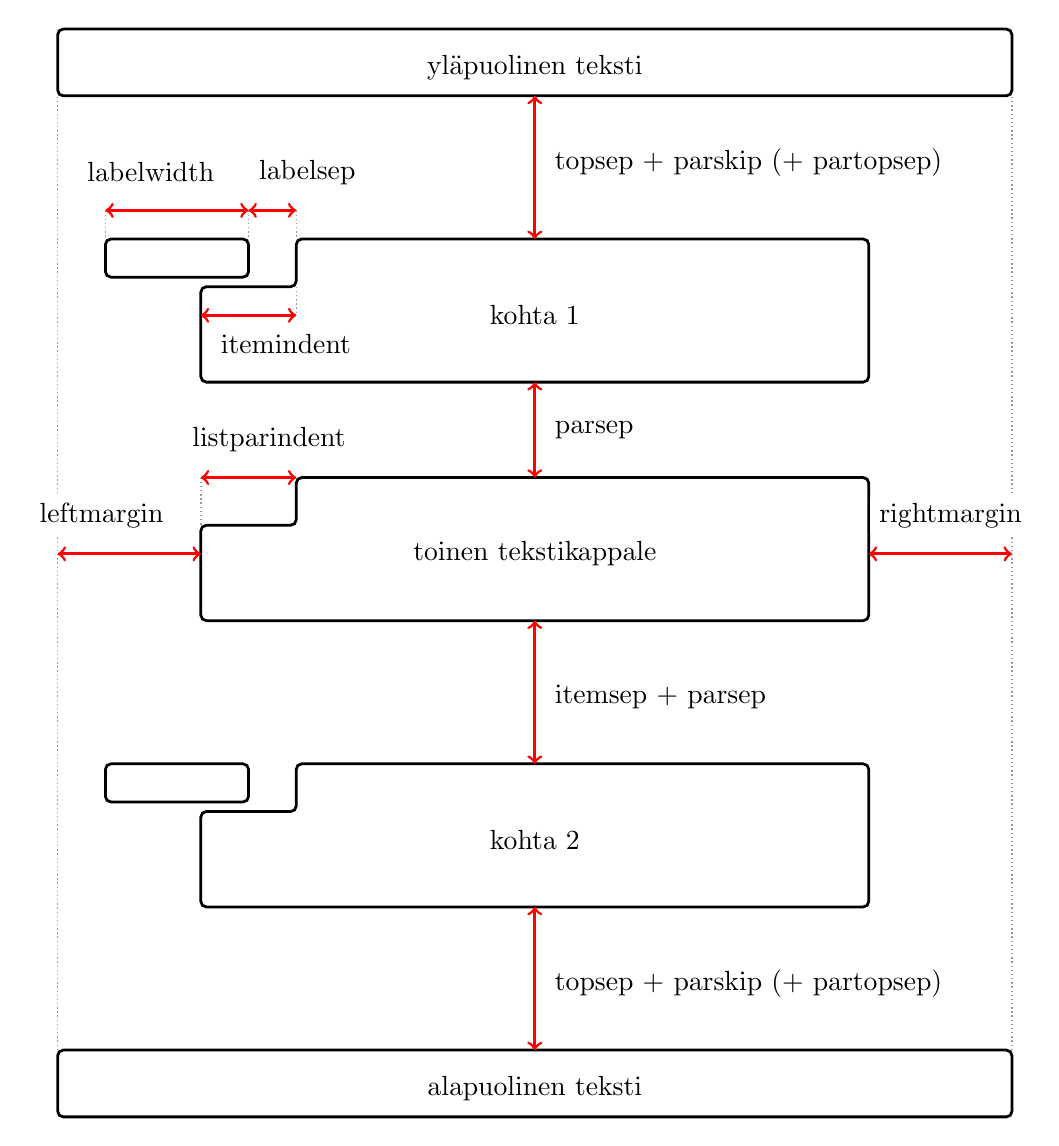
\begin{tikzpicture}
    [x=.01\textwidth, y=.01\textwidth, line width=1bp, rounded corners=2bp]

    \newcommand{\kpl}[1]{\draw (15,#1) -- ++(70,0) -- ++(0,15)
      -- ++(-60,0) -- ++(0,-5) -- ++(-10,0) -- cycle}
    \newcommand{\nuoli}[2]{\draw [color=red, <->] (#1) -- (#2)}
    \newcommand{\kyltti}[2]{\draw (#1) node [anchor=west, fill=white,
      baseline=0bp] {#2}}

    \newcommand{\katko}[2]{\draw [color=black!40, densely dotted, line
      width=.5bp] (#1) -- (#2)}

    \katko{0,10}{0,110};
    \katko{100,10}{100,110};

    \kpl{80};
    \kpl{55};
    \kpl{25};

    \draw (0,10) rectangle ++(100,-7);
    \node at (50,6) {alapuolinen teksti};

    \draw (0,110) rectangle ++(100,7);
    \node at (50,113) {yläpuolinen teksti};

    \nuoli{50,110}{50,95};
    \kyltti{51,103}{\mitta{topsep} + \mitta{parskip} (+ \mitta{partopsep})};

    % Ylin kappale
    \node at (50,87) {kohta 1};
    \draw (5,91) rectangle ++(15,4);
    \katko{5,98}{5,95};
    \katko{20,98}{20,95};
    \katko{25,98}{25,95};
    \nuoli{5,98}{20,98}; \kyltti{2,102}{\mitta{labelwidth}};
    \nuoli{20,98}{25,98}; \kyltti{20,102}{\mitta{labelsep}};
    \katko{25,90}{25,87};
    \nuoli{15,87}{25,87}; \kyltti{16,84}{\mitta{itemindent}};

    \nuoli{50,70}{50,80};
    \kyltti{51,75}{\mitta{parsep}};

    % Keskimmäinen kappale
    \node at (50,62) {toinen tekstikappale};
    \nuoli{0,62}{15,62};
    \kyltti{-3,66}{\mitta{leftmargin}};
    \nuoli{85,62}{100,62};
    \kyltti{85,66}{\mitta{rightmargin}};
    \katko{15,70}{15,65};
    \nuoli{15,70}{25,70};
    \kyltti{13,74}{\mitta{listparindent}};

    \nuoli{50,40}{50,55};
    \kyltti{51,47}{\mitta{itemsep} + \mitta{parsep}};

    % Alin kappale
    \node at (50,32) {kohta 2};
    \draw (5,36) rectangle ++(15,4);

    \nuoli{50,25}{50,10};
    \kyltti{51,17}{\mitta{topsep} + \mitta{parskip} (+ \mitta{partopsep})};
\end{tikzpicture}
}{
  \caption{Luetelmien tekemiseen tarkoitetun \ymparisto{list}\-/
    ympäristön mitat}
  \label{kuva:list-mitat}
}

% Selvitä \makelabel, joka ohjaa luetelmamerkkien latomista.

\section{Taulukot}
\label{luku:taulukot}

...

% \newline \\ \\*

\section{Leijuvat osat}
\label{luku:leijuosat}

...

% \listoffigures, \listoftables, omat listat
% \listoffigurename, \listoftablename

\section{Ristiviitteet}
\label{luku:ristiviitteet}

...

\section{Alaviitteet}
\label{luku:alaviitteet}

...

% geometry: footnotesep

% hyperfootnotes=false, koska muuten footmisc-paketin jotkin asiat eivät
% toimi.

\section{Palstat}
\label{luku:palstat}

% Käsitellään Latexin omat ja multicol-paketti erikseen.

...

\section{Lähdeluettelo ja lähdeviitteet}
\label{luku:lähteet}

Samoin kuin ristiviitteissäkin (luku \ref{luku:ristiviitteet}) Latex
sisältää komennot, joilla lähdeluettelossa mainittuihin teoksiin voidaan
viitata muualta tekstistä. Ajatus on se, että lähdeluettelo laaditaan
tiettyjen komentojen avulla niin, että jokainen lähdeteos saa jonkin
yksilöllisen tunnisteen. Muualta tekstistä viitataan lähdeteoksiin
käyttämällä samoja tunnisteita, ja Latex osaa automaattisesti poimia
lähdeluettelosta esimerkiksi teoksen tekijöiden nimet ja vuosiluvun.

Lähdeviittauksiin ja lähdemerkintöihin on useita käytäntöjä, jotka
vaihtelevat eri ammatti\-/\ ja tieteenaloilla, oppilaitoksilla tai
julkaisijoilla. Tässä yhteydessä käsitellään melko vakiintuneita
suomalaisia käytäntöjä, jotka kuvataan \emph{Kielitoimiston
  oikeinkirjoitusoppaassa} \parencite{kt_oik}. Samalla käsitellään
joitakin asetuksia, joilla kukin voi muokata viittausten ulkoasua omiin
tarpeisiin sopivaksi.

Latex sisältää lähdeluetteloiden ja \=/viittausten perustoiminnot, mutta
niiden avulla ei saa yleisen suomalaisen käytännön mukaisia
lähdeviittauksia. Siksi käytämme apuna makropakettia, jolla viittausten
ja lähdeluettelon ulkoasuun voi vaikuttaa. Ensin käsiteltävä paketti
\paketti{natbib} (luku \ref{luku:natbib}) soveltuu perustarpeisiin ja
lienee sopivin valinta useimmille kirjoittajille. Laajoja tieteellisiä
teoksia kirjoittavan kannattanee opetella käyttämään monipuolista
\paketti{biblatex}\-/pakettia (luku \ref{luku:biblatex}) ja ylläpitää
yhteistä lähdeteosten tietokantaa, josta tarvittavat teokset poimitaan
kunkin dokumentin lähdeluetteloon automaattisesti.

\subsection{Peruskäyttöön (natbib)}
\label{luku:natbib}

Makropaketti \paketti{natbib}\avctan{natbib} laajentaa Latexin
lähdeviittausten perustoimintoja sen verran, että lähteisiin voidaan
viitata teoksen tekijöiden nimen ja vuosiluvun avulla. Seuraava
esimerkki havainnollistaa paketin käyttöönottoa ja asetuksia.

\komentoi{usepackage}
\pakettii{natbib}
\komentoi{setcitestyle}
\begin{koodilohkosis}
  \usepackage{natbib}
  \setcitestyle{authoryear,aysep={},notesep={: }}
\end{koodilohkosis}

Edellisessä esimerkissä viittaustyyli valitaan \komento{setcitestyle}\-/
komennon argumentissa valitsimella \koodi{author\-year}
(tekijä\--vuosi). Valitsimella \koodi{aysep} määritetään, mikä
välimerkki ladotaan tekijän nimen ja vuosiluvun väliin. Tässä se
jätetään tyhjäksi \koodi{\{\}}. \koodi{note\-sep}\-/ valitsimella
asetetaan merkit, jotka ladotaan vuosiluvun ja sitä seuraavan
huomautuksen kuten sivunumeroiden väliin; tässä tapauksessa määritettiin
kaksoispiste ja väli \koodi{\{:~\}}, mutta pilkkukin on yleinen
käytäntö. \komento{setcitestyle}\-/ komennon valitsimet erotetaan
toisistaan pilkulla, eikä erotinpilkkujen ympärillä saa olla
välilyöntejä. Lopputuloksena lähdemerkinnät näyttävät esimerkiksi
seuraavanlaisilta:

\komentoi{citet*}
\begin{koodilohkosis}
  \citet*[27--29]{johdatus} % Viittaus teokseen ”johdatus”.
\end{koodilohkosis}

\begin{tulossis}
  Meikäläinen \& Teikäläinen (2020: 27--29)
\end{tulossis}

Lähdeluettelo kirjoitetaan \ymparistom{thebibliography}\-/ ympäristön ja
\komentom{bibitem}\-/ komentojen avulla esimerkin
\ref{esim:thebibliography} tavoin. Ympäristön aloittavan komennon
(rivi~1) yhteydessä on argumentti \koodi{00}, jolla ei ole tässä
yhteydessä merkitystä. Jos lähdeviittauksen tyylinä olisi
\koodi{numbers} (eikä \koodi{author\-year}), lähdeluettelon teokset
numeroitaisiin, ja silloin \ymparisto{thebibliography}\-/ ympäristön
argumentti ilmaisee, kuinka leveän sisennyksen numeroidut teokset
tarvitsevat. Argumentiksi voi kirjoittaa mitä tahansa merkkejä, ja Latex
mittaa niiden leveyden. Kannattaa kirjoittaa leveitä numeroita kuten
nollia (\koodi{0}) niin monta kappaletta kuin on numeroita suurimmassa
lähdemerkinnän luvussa. Yksi nolla riittää, jos lähteitä on 1--9
kappaletta, kaksi jos lähteitä on kaksinumeroinen määrä eli 10--99
kappaletta jne.

\begin{esimerkki*}
  \ymparistoi{thebibliography}
  \komentoi{bibitem}

\begin{koodilohko}
  \begin{thebibliography}{00}

  \bibitem[Meikäläinen ym.(2020)Meikäläinen \& Teikäläinen]{johdatus}
    Meikäläinen, Matti \& Teikäläinen, Teija (2020): Johdatus alkeiden
    perusteisiin. Toinen painos. Kustantaja Oy.

  \bibitem[Itkonen(2019)]{typografia} Itkonen, Markus (2019):
    Typografian käsikirja. Viides, tarkistettu painos. Typoteekki.
    Graafinen suunnittelu Markus Itkonen Oy.

  \end{thebibliography}
\end{koodilohko}
\caption{Lähdeluettelon kirjoittaminen \ymparisto{thebibliography}\-/
  ympäristön ja \komento{bibitem}\-/ komentojen avulla.}
\label{esim:thebibliography}
\end{esimerkki*}

Komennolla \komento{bibitem} tehdään varsinaiset teosmerkinnät. Samalla
määritetään teoksen yksilöllinen tunniste ja mitä tietoja
lähdeviittauksissa näytetään. Yleinen muoto on seuraavanlainen:

\komentoi{bibitem}
\begin{koodilohkosis}
  \bibitem[lyhyt(vuosi)pitkä]{tunniste} Lähdeluettelon tekstit.
\end{koodilohkosis}

Valinnaisen argumentin aluksi kirjoitetaan lähdeviittauksen lyhyt
merkintä, joka tulisi näkymään lähdeviittauksissa esimerkiksi muodossa
''Meikäläinen ym.''. Heti sen perään kirjoitetaan sulkeissa teoksen
vuosiluku ja sen perään vapaavalintainen lähdeviittauksen pitkä
merkintä, joka näkyisi esimerkiksi tekstinä ''Meikäläinen \&
Teikäläinen''. Vuosiluvun sulkeiden ympärillä ei saa olla välilyöntejä.

Komennon pakollinen argumentti on kyseisen lähdeteoksen yksilöllinen
tunniste, jonka avulla kyseiseen teokseen viitataan. Komennon
argumenttien jälkeen kirjoitetaan samaan tekstikappaleeseen teksti, joka
tulee näkymään lähdeluettelossa.

Lähdeteoksiin viittaamiseen on useita eri komentoja, jotka eroavat
toisistaan siinä, mitä tietoa lähdeviittauksessa näytetään ja onko
lähdeviittaus tai sen osa sulkeissa vai ei. Taulukossa
\ref{tlk:natbib-cite} on joitakin \paketti{natbib}\-/paketin
viittauskomentoja sekä esimerkki viittauksen ulkoasusta. Kuviteltu
esimerkkiteos on peräisin esimerkistä \ref{esim:thebibliography}.

\providecommand{\rivi}{}
\renewcommand{\rivi}[2]{\komento[\{\ldots\}]{#1} & #2 \\}

\leijutlk{
  \begin{tabular}{ll}
    \toprule
    \ots{Komento} & \ots{Esimerkki} \\
    \midrule
    \rivi{citet}{Meikäläinen ym. (2020)}
    \rivi{citet*}{Meikäläinen \& Teikäläinen (2020)}
    \rivi{citep}{(Meikäläinen ym. 2020)}
    \rivi{citep*}{(Meikäläinen \& Teikäläinen 2020)}
    \rivi{citealt}{Meikäläinen ym. 2020}
    \rivi{citealt*}{Meikäläinen \& Teikäläinen 2020}
    \rivi{citeauthor}{Meikäläinen ym.}
    \rivi{citeauthor*}{Meikäläinen \& Teikäläinen}
    \rivi{citeyear}{2020}
    \rivi{citeyearpar}{(2020)}
    \bottomrule
  \end{tabular}
}{
  \caption{\paketti{natbib}\-/paketin lähdeviittauskomentoja}
  \label{tlk:natbib-cite}
}

Lähdeluettelon ulkoasuun voi vaikuttaa mittojen \mittam{bibhang} ja
\mittam{bibsep} avulla. Ensin mainittu on lähdemerkinnän vaakasuuntaisen
riippuvan sisennyksen suuruus, ja jälkimmäinen on lähdemerkintöjen
välinen pystysuuntainen tila. Mitat asetetaan tavalliseen tapaan
\komento{setlength}\-/ komennolla (luku \ref{luku:mitat}):

\komentoi{setlength}
\mittai{parindent}
\mittai{bibhang}
\mittai{bibsep}
\begin{koodilohkosis}
  \setlength{\parindent}{1.1em} % tekstikappaleiden 1. rivin sisennys
  \setlength{\bibhang}{\parindent}
  \setlength{\bibsep}{.5ex plus .1ex minus .1ex}
\end{koodilohkosis}

Lähdemerkintöjen fonttiin voi vaikuttaa määrittelemällä uudelleen
komennon \komentom{bibfont} ja sijoittamalla halutut fontti- tai muut
komennot kyseisen komennon määritelmään.

\komentoi{renewcommand}
\komentoi{bibfont}
\begin{koodilohkosis}
  \renewcommand{\bibfont}{\sffamily\small}
\end{koodilohkosis}

Oletuksena \ymparisto{thebibliography}\-/ ympäristö latoo
lähdeluettelolle otsikon, ja otsikon teksti määräytyy kieliasetusten
(luku \ref{luku:kieliasetukset}) ja dokumenttiluokan perusteella (luku
\ref{luku:dokumenttiluokat}). Suomenkielisen lähdeluettelon otsikon voi
määrittää dokumentin esittelyosassa seuraavan esimerkin tavoin.
Esimerkissä hyödynnetään \komento{addto}\-/ komentoa, joka sisältyy
\paketti{polyglossia}\-/{} ja \paketti{babel}\-/ paketteihin.

\komentoi{addto}
\komentoi{captionsfinnish}
\komentoi{renewcommand}
\komentoi{refname}
\komentoi{bibname}
\luokkai{article}
\luokkai{book}
\luokkai{report}
\begin{koodilohkosis}
  \addto{\captionsfinnish}{%
    \renewcommand{\refname}{Lähteet} % article-dokumenttiluokka
    \renewcommand{\bibname}{Lähteet} % report- ja book-luokat
  }
\end{koodilohkosis}

On myös mahdollista määritellä koko komentosarja, joka suoritetaan
lähdeluettelon otsikoinnin yhteydessä. Se tehdään määrittelemällä
uudelleen komento \komentom{bibsection}.

\komentoi{renewcommand}
\komentoi{bibsection}
\komentoi{setcounter}
\laskurii{secnumdepth}
\komentoi{section}
\begin{koodilohkosis}
  \renewcommand{\bibsection}{%
    \setcounter{secnumdepth}{-1}
    \section{Lähteet}
  }
\end{koodilohkosis}

Edellisessä esimerkissä komennolla \komento{setcounter} määritetään,
mille otsikkotasolle dokumentin otsikoiden eli lukujen numerointi yltää.
Pieni arvo \mbox{(\koodi{-1})} käytännössä tarkoittaa, että seuraaviin
otsikoihin ei tule numerointia; lähdeluettelon otsikkoon ei numerointia
välttämättä haluta. Komento \komento{section} tekee itse otsikon.

Jos ei halua, että \ymparisto{thebibliography}\-/ ympäristö tekee
otsikon automaattisesti, voi \komento{bibsection}\-/ komennon määrittää
tyhjäksi.

\komentoi{renewcommand}
\komentoi{bibsection}
\begin{koodilohkosis}
  \renewcommand{\bibsection}{}
\end{koodilohkosis}

Tässä alaluvussa on käsitelty lähdeluettelon ja lähdeviitteiden
tekemistä \paketti{natbib}\-/paketin toimintojen avulla. Paketti
sisältää muitakin ominaisuuksia, joihin kannattaa tutustua paketin
ohjekirjan avulla. On muun muassa mahdollista tehdä lähdeteoksista
tietokanta Bibtex\-/järjestelmän avulla. Jos kuitenkin siihen suuntaan
haluaa edetä, ei kannata käyttää \paketti{natbib}\-/pakettia eikä
Bibtexiä vaan monipuolisempaa pakettia \paketti{biblatex}, jota
käsitellään seuraavassa alaluvussa.

\subsection{Vaativaan käyttöön (biblatex)}
\label{luku:biblatex}

Suurten lähde- ja kirjallisuusluetteloiden ylläpito voi olla aika
työlästä: pitää jatkuvasti varmistaa, että kaikki viitatut teokset ovat
luettelossa ja että luettelo on pilkulleen yhdenmukainen. Makropaketti
\paketti{biblatex}\avctan{biblatex} on vastaus sellaisiin tarpeisiin.

Ajatuksena on, että kaikki tiedonlähteet ja kirjallisuus kirjoitetaan
tietokantaan, josta \paketti{biblatex}\-/paketin komennot hakevat tiedot
automaattisesti. Kirjoittaja tai työryhmä voi ylläpitää yhtä
kirjallisuustietokantaa, joka voi olla saatavilla oman laitoksen
verkkopalvelimella tai julkisella verkkosivullakin. Dokumentin tekstissä
viitataan teoksiin yksilöllisen tunnisteen avulla, ja pelkän viittauksen
perusteella oikeat teokset ilmestyvät lähdeluetteloon automaattisesti
aakkosjärjestyksessä ja yhdenmukaisessa muodossa. Yhtään tiedonlähdettä
ei tarvitse kirjoittaa lopulliseen lähdeluetteloon käsin.

\paketti{biblatex}\-/paketin käyttö vaatii hieman opettelua -- varsinkin
jos on tarve muokata lähdeluettelon ja lähdeviittausten ulkoasua.
Muutaman tiedonlähteen ylläpito on todennäköisesti paljon helpompaa ja
nopeampaa niillä keinoilla, jotka on kuvattu luvussa \ref{luku:natbib}
(\paketti{natbib}). Sen sijaan laajoja tieteellisiä artikkeleita
kirjoittaville \paketti{biblatex} voi olla suuri apu, koska
artikkeleissa on yleensä paljon lähteitä ja useissakin artikkeleissa
viitataan yleensä samoihin lähteisiin.

\subsubsection{Teostietokanta}

Lähdeteosten tietokanta on erillinen tekstitiedosto, joka tavallisesti
nimetään \koodi{bib}\-/päätteiseksi, esimerkiksi \koodi{teokset.bib}.
Tiedosto koostuu \koodi{@}\=/merkillä ja teostyypin nimellä alkavista
tietueista, joiden yleinen muoto on seuraavanlainen:

\begin{koodilohkosis}
  @teostyyppi{tunniste,
    author = {...},
    title = "..."
  }
\end{koodilohkosis}

Teostyypin nimen jälkeen aaltosulkeiden sisään kirjoitetaan teoksen
kaikki tiedot. Ne alkavat teoksen yksilöllisellä tunnisteella, jota
käytetään lähdeviittauksissa. Tunnisteen jälkeen tulevat muut kentät.
Eri kentät kuten \koodi{author} ja \koodi{title} erotetaan toisistaan
pilkulla. Kentän nimi ja sen sisältö erotetaan toisistaan
yhtäsuuruusmerkillä (\koodi{=}), ja kentän sisältö kirjoitetaan
aaltosulkeiden tai lainausmerkkien sisään, kuten edellinen esimerkki
näyttää.

\begin{esimerkki*}
\begin{koodilohko}
  @book{itkonen_typogr,
    author = {Itkonen, Markus},
    title = {Typografian käsikirja},
    date = {2019},
    edition = {5},
    publisher = {Typoteekki. Graafinen suunnittelu Markus Itkonen Oy}
  }

  @incollection{likonen_teams,
    author = {Likonen, Teemu and Riskilä, Kaisa},
    title = {Verkkoyhteistyö Teams-ympäristössä},
    editor = {Tammi, Tuomo and Horila, Mikko},
    booktitle = {Oppimis- ja toimintaympäristöjen kehittäminen
      harjoittelukouluissa II},
    booksubtitle = {Tilat ja tekniikka pedagogisen kehittämisen tukena},
    publisher = {E-norssi. Opettajankouluttajien yhteistyöverkosto},
    date = {2020},
    pages = {85-92},
    url = {http://www.enorssi.fi/oppimisymparistojulkaisu2020/}
  }

  @article{likonen_tietokanta,
    author = {Likonen, Teemu},
    title = {Tietoa kantaan ja takaisin},
    journaltitle = {Skrolli},
    journalsubtitle = {Tietokonekulttuurin erikoislehti},
    date = {2015},
    volume = {2015},
    number = {4},
    pages = {52-55},
    url = {https://skrolli.fi/numerot/2015-4/}
  }

  @online{ctan,
    title = {Comprehensive TeX Archive Network},
    shorttitle = {CTAN},
    date = {1992/},
    url = {https://www.ctan.org/}
  }
\end{koodilohko}
\caption{Lähdeteosten tietokantatiedosto}
\label{esim:bib-tiedosto}
\end{esimerkki*}

Todellista käyttöä vastaava tietokanta tai sen osa on esimerkissä
\ref{esim:bib-tiedosto}, jossa on neljä erityyppistä teostietuetta:
\koodim{book}, \koodi{incollection}, \koodi{article} ja \koodi{online}.
Ensin mainittu teostyyppi \koodi{book} sopii tavallisille kirjoille,
joissa tietyt tekijät (\koodi{author}) vastaavat suunnilleen koko
teoksen sisällöstä ja teoksella on jokin julkaisijataho
(\koodi{publisher}).

Teostyyppi \koodim{incollection} tarkoittaa esimerkiksi
artikkelikokoelmaa, jonka yksittäiseen artikkeliin (\koodi{title}) ja
sen kirjoittajaan (\koodi{author}) on tarkoitus viitata. Voidaan mainita
myös artikkelin alku- ja loppusivut (\koodi{pages}). Kokoelmalla on
toimittaja (\koodi{editor}) ja yhteinen nimi (\koodi{book\-title}).

Tyyppi \koodim{article} sopii säännöllisesti julkaistavan aikakaus- tai
muun lehden artikkeleihin. Viittauskohteena on yksittäinen artikkeli ja
sen kirjoittaja. Julkaisutiedoissa mainitaan lehden nimi
(\koodi{jour\-nal\-title}), julkaisukausi (\koodi{vol\-ume}), kauteen
kuuluvan julkaisun järjestysnumero (\koodi{num\-ber}) sekä mahdollisesti
artikkelin sivut (\koodi{pages}).

Verkkolähteiden merkitsemiseen sopii \koodim{online}\-/ teostyyppi,
joissa on tavanomaisten kenttien lisäksi ainakin verkko\-/osoite eli
\koodi{url}\-/kenttä ja mahdollisesti viittauspäivä (\koodi{url\-date})
osoittamassa, milloin viitatut tiedot olivat saatavilla.

Teostyyppejä ja teoksiin liittyviä tietokenttiä on olemassa paljon
muitakin. Niiden merkitystä ja käyttöä neuvotaan tarkemmin
\paketti{biblatex}\-/paketin ohjeissa. Seuraavassa on kuitenkin pari
huomiota tietokannan ja kenttien kieliopillisista asioista.

Tietueissa joidenkin kenttien sisältö voi koostua useasta osasta kuten
saman teoksen eri tekijöistä. Eri tekijöiden nimet erotetaan
\koodi{author}- ja \koodi{editor}\-/kentissä toisistaan
\koodi{and}\-/sanalla. Oletuksena \paketti{biblatex} katsoo, että
tekijät ovat henkilöitä, ja käsittelee esimerkiksi etu- ja sukunimet
tietyllä tavalla: jos mukana on pilkku, sitä ennen on sukunimi, ja
etunimet tulevat pilkun jälkeen; jos pilkkua ei ole, etunimet ovat
ensin, ja sukunimi on lopussa.

Jos kuitenkin teoksen tekijänä on yritys tai yhteisö, täytyy sen nimi
kirjoittaa kokonaan aaltosulkeisiin, jottei sitä tulkittaisi
henkilönnimeksi. Tällaisten aaltosulkeiden sisällä voi käyttää
\koodi{and}\-/ sanaa normaalisti, eikä sitä tulkita eri tekijöiden
erottimeksi. Seuraavassa on näistä esimerkit:

\begin{koodilohkosis}
  author = {Meikäläinen, Matti and Teikäläinen, Teija}
  author = {{Org. of Latex and Typography} and Meikäläinen, Matti}
\end{koodilohkosis}

Muunkinlaisia useasta osasta koostuvia kenttiä on olemassa.
Asiasanakentän (\koodi{keywords}) eri sanat erotetaan toisistaan
pilkulla, ja sivunumeroissa (\koodi{pages}) voi olla myös lukualueita,
jotka ilmaistaan yhdysmerkillä~\mbox{(\koodi{-})}.

\begin{koodilohkosis}
  keywords = {eri, sanoja, peräkkäin}
  pages = {15-19}
\end{koodilohkosis}

Teostietokantaan voi määrittää vakiosisältöisiä muuttujia käyttämällä
\koodi{@string}\-/ rakennetta. Vakioihin voi sitten viitata
teostietueiden kentistä esimerkin \ref{esim:bib-muuttujat} tavoin.
Vakiot ovat hyödyllisiä silloin, kun sama kentän sisältö toistuu useissa
teoksissa, kuten tässä esimerkissä sama tekijä (\koodi{author}) ja
aikakauslehden nimi (\koodi{jour\-nal\-title}). Vakioita voi yhdistää
saman kentän muuhun sisältöön käyttämällä \koodi{\#}\=/merkkiä, kuten
esimerkin rivillä 13 on tehty.

\begin{esimerkki*}
\begin{koodilohko}
  @string{
    oma = {Meikäläinen, Matti},
    lehti = {Hienon hieno aikakauslehti}
  }

  @article{hieno_artikkeli,
    author = oma,
    journaltitle = lehti,
    ...
  }

  @article{toinen_artikkeli,
    author = oma # { and Teikäläinen, Teija},
    journaltitle = lehti,
    ...
  }
\end{koodilohko}
\caption{Muuttujien käyttö ja \koodi{@string}\-/rakenne}
\label{esim:bib-muuttujat}
\end{esimerkki*}

\subsubsection{Käyttöönotto}

\paketti{biblatex}\-/makropaketti otetaan käyttöön esimerkin
\ref{esim:biblatex-käyttöönotto} rivien avulla. Mukana ovat myös paketit
\paketti{polyglossia} ja \paketti{csquotes}. Jälkimmäinen sisältää
lainausmerkkien käyttöön liittyvää logiikkaa (luku
\ref{luku:lainausmerkit}), jota ilman \paketti{biblatex} ei saa eri
kielten erilaisia lainausmerkkejä oikein vaan käyttää pelkästään
amerikkalaisia (``~'').

\begin{esimerkki*}
  \komentoi{usepackage}
  \pakettii{polyglossia}
  \pakettii{csquotes}
  \pakettii{biblatex}

\begin{koodilohko}
  % Polyglossia tai babel on ladattava ennen biblatexia.
  \usepackage{polyglossia}

  % Kielikohtaiset lainausmerkit oikein csquoten avulla.
  \usepackage{csquotes}

  \usepackage[style=authoryear]{biblatex}
\end{koodilohko}
\caption{\paketti{biblatex}\-/ makropaketin käyttöönotto ja asetuksia}
\label{esim:biblatex-käyttöönotto}
\end{esimerkki*}

Paketin asetuksissa käytetään valitsinta \koodi{style} ja sen asetusta
\koodi{author\-year}, joka asettaa lähdeviittausten ja lähdeluettelon
tyyliksi tekijän ja vuosiluvun. Se on yleinen käytäntö suomenkielisissä
teksteissä. Vastaavia tyylejä ovat myös \koodi{author\-year-comp},
\koodi{author\-year-ibid} ja \koodi{author\-year-icomp}, jotka lisäksi
tiivistävät peräkkäisiä lähdeviittauksia, jos teoksen tekijä on sama.

Numerointiin tai kirjainlyhenteisiin perustuvat lähdeluettelo\-/{} ja
viittaustyylit ovat nimeltään \koodi{nu\-mer\-ic} ja
\koodi{al\-pha\-bet\-ic}. Muitakin tyylejä on olemassa, mutta tämän
oppaan esimerkeissä käsitellään tekijä--vuosi-tyyliä.

Makropaketin omien lähdeluettelo\-/{} ja viittaustyylien lisäksi
Latex\-/jakelupaketissa on todennäköisesti mukana myös ulkopuolisten
tahojen tekemiä tyylejä. Tyylikokonaisuus nimeltä
\paketti{biblatex-ext}\avctan{biblatex-ext} laajentaa
\paketti{biblatex}\-/paketin tavallisten tyylien ominaisuuksia.
Laajennettujen tyylien käyttäminen ei vaadi erillisen makropaketin
lataamista, vaan tyylin saa käyttöön yksinkertaisesti vain
kirjoittamalla sen nimen \paketti{biblatex}\-/paketin lataamisen
yhteydessä. Laajennetut tyylit alkavat kirjaimilla \mbox{\koodi{ext-},}
esimerkiksi \koodi{ext-author\-year} tai \koodi{ext-author\-year-comp}.

Esimerkin \ref{esim:biblatex-käyttöönotto} komentojen lisäksi täytyy
komennolla \komento{addbibresource} nimetä kaikki käyttöön otettavat
teostietokantatiedostot. Komentoja ja tiedostoja voi olla useampiakin,
ja tietokanta voi olla myös verkko\-/osoitteen takana oleva tiedosto.
\komento{addbibresource}\-/ komennot täytyy kirjoittaa Latex\-/
dokumentin esittelyosaan.

\komentoi{addbibresource}
\begin{koodilohkosis}
  \addbibresource{teokset.bib}
  \addbibresource{~/texmf/omat_kirjoitukset.bib}
  \addbibresource[location=remote]{http://osoite.netissä/yhteiset.bib}
\end{koodilohkosis}

Lähdeluettelo ladotaan dokumenttiin komennolla
\komento{printbibliography}. Komennolle voi antaa valinnaisen
argumentin, jonka valitsimilla vaikutetaan esimerkiksi lähdeluettelon
otsikon tekstiin tai poistetaan automaattinen otsikointi kokonaan. On
myös olemassa erilaisia lähdeteosten rajaamisvalitsimia, joiden avulla
voi määrittää, mitä teoksia kyseiseen luetteloon halutaan. Näin voidaan
esimerkiksi rajata painetut lähteet yhteen luetteloon, julkaisemattomat
toiseen ja verkkolähteet kolmanteen.

\komentoi{printbibliography}
\begin{koodilohkosis}
  \printbibliography
  \printbibliography[title={Lähteet}]
  \printbibliography[heading=none,  % Ei automaattista otsikkoa,
    type=online]           % ja rajataan vain online-tyyppisiin.
\end{koodilohkosis}

Lähdeluetteloon tulevat mukaan vain ne teokset, joihin on viitattu.
Mitään ei siis näy, jos ei ole lähdeviittauksia. Seuraavassa alaluvussa
käsitellään lähdeviittauskomentoja ja myös ''näkymätöntä''
viittauskomentoa, jolla teoksia saadaan mukaan luetteloon ilman näkyvää
viittausta.

\subsubsection{Lähdeviittaukset}

\providecommand{\rivi}{}
\renewcommand{\rivi}[2]{\komento[\{\ldots\}]{#1} & #2 \\}

\leijutlk{
  \begin{tabular}{ll}
    \toprule
    \ots{Komento} & \ots{Esimerkki} \\
    \midrule
    \rivi{cite}{Meikäläinen 2020}
    \rivi{textcite}{Meikäläinen (2020)}
    \rivi{parencite}{(Meikäläinen 2020)}
    \rivi{citeauthor}{Meikäläinen}
    \rivi{citeyear}{2020}
    \rivi{citetitle}{[teoksen nimi]}
    \rivi{footcite}{Meikäläinen 2020 [alaviitteessä]}
    \rivi{nocite}{[näkymätön viittaus]}
    \bottomrule
  \end{tabular}
}{
  \caption{\paketti{biblatex}\-/paketin lähdeviittauskomentoja}
  \label{tlk:biblatex-cite}
}

Taulukkoon \ref{tlk:biblatex-cite} on koottu tavallisimpia
\paketti{biblatex}\-/paketin viittauskomentoja. Komennoille voi antaa
valinnaisen argumentin, jolla kerrotaan täsmentävää tietoa
lähdeviittauksesta. Yleensä se on viitattavan teoksen sivunumero.
Viittaus näkyy dokumentissa esimerkiksi seuraavalla tavalla:

\komentoi{textcite}
\begin{koodilohkosis}
  \textcite[27--29]{johdatus} % Viittaus teokseen ”johdatus”.
\end{koodilohkosis}

\begin{tulossis}
  Meikäläinen ja Teikäläinen (2020, s. 27--29)
\end{tulossis}

Jos halutaan sisällyttää lähdeluetteloon teoksia, joihin ei ole
välttämättä viitattu, käytetään dokumentissa kerran ''näkymätöntä''
viittauskomentoa \komento{nocite}. Sille annetaan argumentiksi
tunnisteet niistä teoksista, jotka halutaan mukaan luetteloon.
Argumentti~\koodi{*} (tähti) valitsee kaikki teokset.

\komentoi{nocite}
\begin{koodilohkosis}
  \nocite{meikäläinen, teikäläinen} % Nämä teokset mukaan.
  \nocite{*}                        % Kaikki mukaan.
\end{koodilohkosis}

\subsubsection{Lähdetiedostojen kääntäminen}

Latexin kääntäjäohjelmat Lualatex tai Xelatex eivät yksinään riitä,
sillä teostietokanta ei ole tavallinen Latex\-/muotoinen tiedosto.
Tarvitaan myös Latex\-/jakelun mukana tulevaa komentoa \koodi{biber},
joka käsittelee teostietokantaan liittyviä tiedostoja. Lopulta
Latex\-/kääntäjääkin täytyy kutsua kaksi kolme kertaa, jotta kaikki
ristiviitteet saadaan kuntoon. Komentojen suoritusjärjestys on
seuraavanlainen:

\begin{koodilohkosis}
  lualatex teksti.tex
  biber teksti.bcf
  lualatex teksti.tex
  lualatex teksti.tex
\end{koodilohkosis}

Edellisen esimerkin komennoissa voi tiedoston nimistä jättää päätteet
pois (\koodi{.tex}, \koodi{.bcf}). \koodi{lualatex}\-/ ohjelman paikalla
voi olla myös \koodi{xelatex}. Kääntäminen on vielä helpompaa, kun
käyttää \koodi{latexmk}\-/ ohjelmaa (luku \ref{luku:latexmk}), joka osaa
automaattisesti suorittaa myös \koodi{biber}\-/ ohjelman ja tarvittavat
uudelleen kääntämiset. Yksi komento riittää käyttäjälle:

\begin{koodilohkosis}
  latexmk -lualatex teksti.tex    % tai: -xelatex
\end{koodilohkosis}

\subsubsection{Lähdeluettelon mittoja}

Lähdeluettelon ulkoasuun voi vaikuttaa muutaman eri mitan avulla, joista
esitellään tässä yhteydessä vain osa. Lähdemerkinnän riippuvan
sisennyksen suuruus määräytyy mitan \mittam{bibhang} avulla. Yleensä
lienee sopivaa asettaa se samaksi kuin tekstikappaleiden ensimmäisen
rivin sisennys \mitta{parindent}.

\komentoi{setlength}
\mittai{parindent}
\mittai{bibhang}
\begin{koodilohkosis}
  \setlength{\parindent}{1.1em} % tekstikappaleiden 1. rivin sisennys
  \setlength{\bibhang}{\parindent}
\end{koodilohkosis}

Mitta \mitta{bibitemsep} on lähdemerkintöjen välinen pystysuuntainen
tila. \mittamargin{bibitemsep} Sen avulla voi harventaa lähdeluetteloa,
jolloin lähdemerkinnät erottuvat paremmin toisistaan. Mitan
\mittam{bibnamesep} avulla voi tehdä suuremman pystysuuntaisen välin
lähdemerkintöjen väliin silloin, kun teoksen tekijä vaihtuu
(\koodi{author} tai \koodi{editor}). Toisin sanoen tämän mitan avulla
voi ryhmitellä saman tekijän teokset tiiviimmin yhteen ja jättää väliä
seuraavan tekijän teoksiin. Vastaavanlainen mitta on
\mittam{bibinitsep}, jota käytetään silloin, kun lähdemerkinnän
aloittava kirjain vaihtuu. Tämän avulla voi ryhmitellä lähdemerkinnät
aakkosittain eli tehdä suuremman välin aina lähdemerkinnän alkukirjaimen
vaihtuessa.

\komentoi{setlength}
\mittai{bibitemsep}
\mittai{bibnamesep}
\mittai{bibinitsep}
\begin{koodilohkosis}
  \setlength{\bibitemsep}{.5ex plus .1ex minus .1ex}
  \setlength{\bibnamesep}{1em  plus .2ex minus .1ex}
  \setlength{\bibinitsep}{2em  plus .2ex minus .1ex}
\end{koodilohkosis}

\subsubsection{Muita asetuksia}

Lähdemerkintöjen fonttiin voi vaikuttaa määrittelemällä uudelleen
komennon \komentom{bibfont} ja sijoittamalla halutut fontti- tai muut
komennot kyseisen komennon määritelmään.

\komentoi{renewcommand}
\komentoi{bibfont}
\begin{koodilohkosis}
  \renewcommand{\bibfont}{\sffamily\small}
\end{koodilohkosis}

Lähdemerkinnät itsessään muodostetaan automaattisesti tiettyjen
tyyliasetusten perusteella. Omiakin tyylejä voi tehdä, mutta yleensä
riittää vain yksittäisen asetusten muuttaminen. Niistä käsitellään tässä
yhteydessä muutama. Asetusten muuttamiseen tarvitaan yleensä
\paketti{biblatex}\-/ paketin omia asetuskomentoja.

Lähdeluettelon nimet näkyvät oletusasetuksilla siten, että teoksen
ensimmäisen tekijän sukunimi mainitaan ensin (luettelon
aakkosjärjestyksen vuoksi) mutta saman teoksen muiden tekijöiden etunimi
mainitaan ensin. Tekijöiden nimet näkyvät siis seuraavalla tavalla:
''Meikäläinen, Matti ja Teija Teikäläinen''. Suomessa on kuitenkin
tapana kirjoittaa kaikki nimet samalla tavalla ja mainita sukunimi aina
ensin. Tämä saadaan toteutettua seuraavilla komennolla:

\komentoi{DeclareNameAlias}
\begin{koodilohkosis}
  \DeclareNameAlias{default} {family-given}
  \DeclareNameAlias{sortname}{family-given}
\end{koodilohkosis}

\begin{tulossis}
  Meikäläinen, Matti ja Teikäläinen, Teija (2020). --~--
\end{tulossis}

Saman teoksen eri tekijöiden nimet erotetaan oletuksena toisistaan
pilkuilla paitsi kahden viimeisen nimen välissä on \textit{ja}-sana.
Usein on kuitenkin tapana käyttää \&\=/merkkiä ainakin lähdeluettelossa.
Seuraavat esimerkkikomennot asettavat lähdeluettelon kaikkien nimien
erottimeksi \&\=/merkin.

\komentoi{DeclareDelimFormat}
\begin{koodilohkosis}
  \DeclareDelimFormat[bib]{multinamedelim}{\space\&\space}
  \DeclareDelimFormat[bib]{finalnamedelim}{\space\&\space}
\end{koodilohkosis}

\begin{tulossis}
  Meikäläinen, Matti \& Teikäläinen, Teija \& Tutkija, Tuija (2020).
  --~--
\end{tulossis}

Erotinmerkkiasetuksen nimi \koodi{multi\-name\-delim} tarkoittaa muiden
kuin kahden viimeisen tekijän nimen välissä olevaa erotinta. Kahden
viimeisen nimen erotin määritellään asetuksella
\koodi{final\-name\-delim}.

Edellisten esimerkkikomentojen valinnainen argumentti \koodi{bib}
tarkoittaa, että vaikutetaan vain lähdeluetteloon. Argumentti voi olla
myös esimerkiksi \koodi{cite}, \koodi{textcite} tai \koodi{parencite},
jolloin vaikutetaan samannimisillä komennoilla tehtyihin
lähdeviittauksiin: \komento{cite}, \komento{textcite} ja
\komento{parencite}. Katso lähdeviittauskomennot taulukosta
\ref{tlk:biblatex-cite}. Seuraava esimerkki vaihtaa
\komento{parencite}\-/ komentoon asetuksen, niin että kahden viimeisen
henkilön nimen väliin ladotaan \&\=/merkki. Oletuksena viittauksissa
käytetään \textit{ja}\-/sanaa.

\komentoi{DeclareDelimFormat}
\begin{koodilohkosis}
  \DeclareDelimFormat[parencite]{finalnamedelim}{\space\&\space}
\end{koodilohkosis}

\begin{tulossis}
  (Meikäläinen, Teikäläinen \& Tutkija 2020)
\end{tulossis}

Useiden saman teoksen tekijöiden luettelot lyhennetään automaattisesti
esimerkiksi muotoon ''Meikäläinen et~al.'', ja lyhentämisen säännöt
määritellään tiettyjen \koodi{max}- ja \koodi{min}\-/alkuisten paketin
valitsimien avulla. Lähdeluettelossa teoksen tekijäluetteloon
vaikutetaan valitsimilla \koodi{max\-bib\-names} ja
\koodi{min\-bib\-names}, kun taas lähdeviittausten tekijäluetteloon
vaikutetaan valitsimilla \koodi{max\-cite\-names} ja
\koodi{min\-cite\-names}. Asetukset toimivat siten, että jos
enimmäismäärä (max) ylittyy, typistetään tekijäluettelo vähimmäismäärään
(min) ja lisätään ilmaus ''et al.'' tms.

Tekijäluetteloa ei kuitenkaan välttämättä lyhennetä, jos luettelosta
tulisi täsmälleen samanlainen kuin jollakin toisella teoksella. Tähän
asiaan puolestaan vaikutetaan valitsimella \koodi{unique\-list}, joka on
oletuksena päällä viittaustyylissä \koodi{author\-year}.

\komentoi{usepackage}
\pakettii{biblatex}
\begin{koodilohkosis}
  \usepackage[style=authoryear, maxbibnames=99, minbibnames=3,
    maxcitenames=3, mincitenames=1, uniquelist=true]{biblatex}
\end{koodilohkosis}

Kun halutaan näyttää lähdeluettelossa vain tekijän etunimen alkukirjain
eikä koko etunimeä, käytetään paketin valitsinta \koodi{given\-inits}.

\komentoi{usepackage}
\pakettii{biblatex}
\begin{koodilohkosis}
  \usepackage[…, giveninits]{biblatex}
\end{koodilohkosis}

\begin{tulossis}
  Meikäläinen, M. (2020). -- --
\end{tulossis}

Lähdeluettelossa näytetään teoksen tekijän nimen kohdalla ajatusviiva,
jos tekijä on sama kuin luettelon edelliselläkin teoksella. Mikäli tätä
(sinänsä yleistä) käytäntöä ei haluta, täytyy käyttää paketin asetusta
\koodi{dash\-ed=\katk false}.

\komentoi{usepackage}
\pakettii{biblatex}
\begin{koodilohkosis}
  \usepackage[…, dashed=false]{biblatex}
\end{koodilohkosis}

Joskus on tapana latoa lähdeluettelossa tekijöiden nimet esimerkiksi
pienversaalilla, jotta ne erottuvat luettelosta paremmin. Tällainen
muutos vaatii, että lähdeluettelon tulostamisen yhteydessä määritellään
uudelleen henkilön nimiin liittyvät tulostuskomennot
\komento{mkbibnamefamily}, \komento{mkbibnamegiven},
\komento{mkbibnameprefix} ja \komento{mkbibnamesuffix}. Se saadaan
automaattiseksi seuraavilla komennoilla:

\komentoi{AtBeginBibliography}
\komentoi{mkbibnamefamily}
\komentoi{mkbibnamegiven}
\komentoi{mkbibnameprefix}
\komentoi{mkbibnamesuffix}
\begin{koodilohkosis}
  \AtBeginBibliography{%
    \renewcommand{\mkbibnamefamily}[1]{\textsc{#1}}
    \renewcommand{\mkbibnamegiven} [1]{\textsc{#1}}
    \renewcommand{\mkbibnameprefix}[1]{\textsc{#1}}
    \renewcommand{\mkbibnamesuffix}[1]{\textsc{#1}}
  }
\end{koodilohkosis}

\begin{tulossis}
  \textsc{Meikäläinen}, \textsc{Matti} \& \textsc{Teikäläinen},
  \textsc{Teija} (2020). -- --
\end{tulossis}

Lähdeluettelon eri osien erottimena on yleensä piste. Joskus kuitenkin
tekijöiden nimien ja vuosiluvun jälkeen halutaan kaksoispiste. Se
saadaan toteutettua seuraavalla komennolla:

\komentoi{DeclareDelimFormat}
\begin{koodilohkosis}
  \DeclareDelimFormat[bib]{nametitledelim}{\addcolon\space}
\end{koodilohkosis}

\begin{tulossis}
  Meikäläinen, Matti (2020): -- --
\end{tulossis}

Oletuksena \paketti{biblatex} kursivoi \koodi{book}\-/ tyyppisten
teosten nimen (\koodi{title}). Sen sijaan artikkelikokoelmissa
(\koodi{incollection}) ja aikakauslehdissä (\koodi{article})
kursivoidaan julkaistun kokoelman nimi (\koodi{book\-title}) ja
aikakauslehden nimi (\koodi{jour\-nal\-title}). Näissä teostyypeissä
viitatun artikkelin nimi (\koodi{title}) kirjoitetaan lainausmerkkeihin.
Käytäntö tuntuu järkevältä, sillä kursivoituna on aina julkaistu
kokonainen teos eikä sen osa. Käytännössähän tiedonlähde joudutaan
hakemaan teoksen nimen perusteella. Joku voi silti haluta muuttaa näiden
ulkoasua ja esimerkiksi kursivoida aina viittauksen kohteena olevan
artikkelin. Seuraavassa on esimerkkikomennot edellä mainittujen
lähdeluettelon kenttien muuttamiseen.

\komentoi{DeclareFieldFormat}
\begin{koodilohkosis}
  \DeclareFieldFormat[article,incollection]{title}{\emph{#1}}
  \DeclareFieldFormat[article]{journaltitle}{#1}
  \DeclareFieldFormat[incollection]{booktitle}{#1}
\end{koodilohkosis}

Edellä olevissa esimerkkikomennoissa on valinnaisena argumenttina ne
teostyypit, joihin halutaan vaikuttaa. Jos valinnaisen argumentin jättää
pois, vaikutetaan kaikkiin teostyyppeihin, ellei tarkempaa
teostyyppikohtaista määritelmää ole olemassa. Ensimmäinen pakollinen
argumentti on kentän nimi teostietokannassa, ja toinen pakollinen
argumentti on sisältö, joka ladotaan lähdemerkintään kyseisen tiedon
kohdalle. Teostietokannasta tulevan kentän sisältö on parametrissa
\koodi{\#1}.

Mikäli haluaa jonkin teoksen tiedon lainausmerkkeihin tai sulkeisiin,
kannattaa käyttää komentoa \komento{mkbibquote} tai
\komento{mkbibparens}. Ne ymmärtävät ottaa huomioon eri kielten
lainausmerkkikäytännöt ja mahdolliset sisäkkäiset sulkeet.

\komentoi{DeclareFieldFormat}
\komentoi{mkbibquote}
\begin{koodilohkosis}
  \DeclareFieldFormat[incollection]{booktitle}{\mkbibquote{#1}}
\end{koodilohkosis}

Oletuksena teoksen vuosiluku tai muu päiväys ladotaan lähdeluetteloon
sulkeissa. Joissakin lähdeluettelokäytännöissä sulkeita ei kuitenkin
ole, joten seuraavaksi käsitellään keino sulkeiden poistamiseen.
Tavallisessa \paketti{biblatex}\-/paketin lähdeluettelotyylissä
\koodi{author\-year} ei ole omaa asetusta teoksen päiväyksen ulkoasun
muuttamiseen, mutta jos käyttää tyyliä \koodi{ext-author\-year} (tms.),
sekin puute korjaantuu, ja voi käyttää \koodi{bib\-label\-date}\-/
asetusta.

\komentoi{usepackage}
\pakettii{biblatex}
\komentoi{DeclareFieldFormat}
\begin{koodilohkosis}
  \usepackage[style=ext-authoryear]{biblatex}

  \DeclareFieldFormat{biblabeldate}{#1}
\end{koodilohkosis}

\begin{tulossis}
  Meikäläinen, Matti 2020. -- --
\end{tulossis}

Artikkelikokoelmissa (teostyyppi \koodi{incollection}) mainitaan
oletuksena kokoelman nimi ja toimittajat seuraavassa muodossa:
''Teoksessa: \textit{Hieno artikkelikokoelma.} Toim. Kirjailija,
Kaisa''. Ensin siis mainitaan julkaisun nimi ja sen jälkeen toimittajien
nimet. Suomessa on tapana kirjoittaa nämä tiedot toisinpäin ja laittaa
toimittajarooli sulkeisiin. Tällaiset asetukset saa käyttämällä tyyliä
\koodi{ext-author\-year} (tms.), paketin asetusta
\koodi{in\-name\-before\-title=\katk true} ja seuraavia komentoja:

\komentoi{usepackage}
\pakettii{biblatex}
\komentoi{DeclareFieldFormat}
\komentoi{DeclareDelimFormat}
\komentoi{mkbibparens}
\begin{koodilohkosis}
  \usepackage[style=ext-authoryear, innamebeforetitle=true]{biblatex}

  \DeclareFieldFormat{editortype}{\mkbibparens{#1}}
  \DeclareDelimFormat{editortypedelim}{\addspace}
\end{koodilohkosis}

\begin{tulossis}
  -- -- Teoksessa: Kirjailija, Kaisa (toim.). \textit{Hieno
    artikkelikokoelma}. -- --
\end{tulossis}

Lähdeviittauksissa vuosiluvun ja sivunumeroiden välissä käytetään
toisinaan pilkkua ja toisinaan kaksoispistettä. Sivunumeroiden
yhteydessä voi olla lyhenne ''s.'' tai se voidaan jättää pois.
Seuraavilla komennoilla vaikutetaan näihin asetuksiin:

\komentoi{DeclareFieldFormat}
\komentoi{DeclareDelimFormat}
\komentoi{textcite}
\begin{koodilohkosis}
  \DeclareFieldFormat{postnote}{#1} % Lyhenne ”s.” pois.
  \DeclareDelimFormat{postnotedelim}{\addcolon\space} % Kaksoispiste.

  \textcite[15--16]{tunniste} toteaa artikkelissaan -- --
\end{koodilohkosis}

\begin{tulossis}
  Meikäläinen (2020: 15--16) toteaa artikkelissaan -- --
\end{tulossis}

Kun saman teoksen usean tekijän luettelo lyhennetään, käytetään
oletuksena latinankielistä ilmausta pois jäävien nimien tilalla:
''Meikäläinen et al.''. Ilmauksen voi muuttaa suomenkieliseksi
seuraavalla komennolla:

\komentoi{DefineBibliographyStrings}
\begin{koodilohkosis}
  \DefineBibliographyStrings{finnish}{
    andothers = {ym.},
  }
\end{koodilohkosis}

\begin{tulossis}
  Meikäläinen ym. (2020)
\end{tulossis}

\paketti{biblatex}\-/paketti sisältää valtavan paljon asetuksia ja
mahdollisuuksia lähdeluettelon ja \=/viitteiden ulkoasun säätämiseen.
Esimerkiksi komennolla \komento{DeclareBibliographyDriver} voi ottaa
täysin haltuun, miten tietty teostyyppi ladotaan lähdeluetteloon.
Komennolla \komento{DeclareSortingTemplate} voi määritellä omia
aakkostustapoja. Lisätietoa saa paketin ohjekirjasta.%
\avctan{biblatex}

\section{Asiahakemisto}
\label{luku:asiasanat}

...

\section{Kuvat}
\label{luku:grafiikka}

...

\section{Diaesitykset}
\label{luku:diaesitykset}

...

\section{Kirjeet}
\label{luku:kirjeet}

...
